\documentclass[english,floatsintext,man]{apa6}

\usepackage{amssymb,amsmath}
\usepackage{ifxetex,ifluatex}
\usepackage{fixltx2e} % provides \textsubscript
\ifnum 0\ifxetex 1\fi\ifluatex 1\fi=0 % if pdftex
  \usepackage[T1]{fontenc}
  \usepackage[utf8]{inputenc}
\else % if luatex or xelatex
  \ifxetex
    \usepackage{mathspec}
    \usepackage{xltxtra,xunicode}
  \else
    \usepackage{fontspec}
  \fi
  \defaultfontfeatures{Mapping=tex-text,Scale=MatchLowercase}
  \newcommand{\euro}{€}
\fi
% use upquote if available, for straight quotes in verbatim environments
\IfFileExists{upquote.sty}{\usepackage{upquote}}{}
% use microtype if available
\IfFileExists{microtype.sty}{\usepackage{microtype}}{}
\usepackage{color}
\usepackage{fancyvrb}
\newcommand{\VerbBar}{|}
\newcommand{\VERB}{\Verb[commandchars=\\\{\}]}
\DefineVerbatimEnvironment{Highlighting}{Verbatim}{commandchars=\\\{\}}
% Add ',fontsize=\small' for more characters per line
\usepackage{framed}
\definecolor{shadecolor}{RGB}{248,248,248}
\newenvironment{Shaded}{\begin{snugshade}}{\end{snugshade}}
\newcommand{\KeywordTok}[1]{\textcolor[rgb]{0.13,0.29,0.53}{\textbf{#1}}}
\newcommand{\DataTypeTok}[1]{\textcolor[rgb]{0.13,0.29,0.53}{#1}}
\newcommand{\DecValTok}[1]{\textcolor[rgb]{0.00,0.00,0.81}{#1}}
\newcommand{\BaseNTok}[1]{\textcolor[rgb]{0.00,0.00,0.81}{#1}}
\newcommand{\FloatTok}[1]{\textcolor[rgb]{0.00,0.00,0.81}{#1}}
\newcommand{\ConstantTok}[1]{\textcolor[rgb]{0.00,0.00,0.00}{#1}}
\newcommand{\CharTok}[1]{\textcolor[rgb]{0.31,0.60,0.02}{#1}}
\newcommand{\SpecialCharTok}[1]{\textcolor[rgb]{0.00,0.00,0.00}{#1}}
\newcommand{\StringTok}[1]{\textcolor[rgb]{0.31,0.60,0.02}{#1}}
\newcommand{\VerbatimStringTok}[1]{\textcolor[rgb]{0.31,0.60,0.02}{#1}}
\newcommand{\SpecialStringTok}[1]{\textcolor[rgb]{0.31,0.60,0.02}{#1}}
\newcommand{\ImportTok}[1]{#1}
\newcommand{\CommentTok}[1]{\textcolor[rgb]{0.56,0.35,0.01}{\textit{#1}}}
\newcommand{\DocumentationTok}[1]{\textcolor[rgb]{0.56,0.35,0.01}{\textbf{\textit{#1}}}}
\newcommand{\AnnotationTok}[1]{\textcolor[rgb]{0.56,0.35,0.01}{\textbf{\textit{#1}}}}
\newcommand{\CommentVarTok}[1]{\textcolor[rgb]{0.56,0.35,0.01}{\textbf{\textit{#1}}}}
\newcommand{\OtherTok}[1]{\textcolor[rgb]{0.56,0.35,0.01}{#1}}
\newcommand{\FunctionTok}[1]{\textcolor[rgb]{0.00,0.00,0.00}{#1}}
\newcommand{\VariableTok}[1]{\textcolor[rgb]{0.00,0.00,0.00}{#1}}
\newcommand{\ControlFlowTok}[1]{\textcolor[rgb]{0.13,0.29,0.53}{\textbf{#1}}}
\newcommand{\OperatorTok}[1]{\textcolor[rgb]{0.81,0.36,0.00}{\textbf{#1}}}
\newcommand{\BuiltInTok}[1]{#1}
\newcommand{\ExtensionTok}[1]{#1}
\newcommand{\PreprocessorTok}[1]{\textcolor[rgb]{0.56,0.35,0.01}{\textit{#1}}}
\newcommand{\AttributeTok}[1]{\textcolor[rgb]{0.77,0.63,0.00}{#1}}
\newcommand{\RegionMarkerTok}[1]{#1}
\newcommand{\InformationTok}[1]{\textcolor[rgb]{0.56,0.35,0.01}{\textbf{\textit{#1}}}}
\newcommand{\WarningTok}[1]{\textcolor[rgb]{0.56,0.35,0.01}{\textbf{\textit{#1}}}}
\newcommand{\AlertTok}[1]{\textcolor[rgb]{0.94,0.16,0.16}{#1}}
\newcommand{\ErrorTok}[1]{\textcolor[rgb]{0.64,0.00,0.00}{\textbf{#1}}}
\newcommand{\NormalTok}[1]{#1}

% Table formatting
\usepackage{longtable, booktabs}
\usepackage{lscape}
% \usepackage[counterclockwise]{rotating}   % Landscape page setup for large tables
\usepackage{multirow}		% Table styling
\usepackage{tabularx}		% Control Column width
\usepackage[flushleft]{threeparttable}	% Allows for three part tables with a specified notes section
\usepackage{threeparttablex}            % Lets threeparttable work with longtable

% Create new environments so endfloat can handle them
% \newenvironment{ltable}
%   {\begin{landscape}\begin{center}\begin{threeparttable}}
%   {\end{threeparttable}\end{center}\end{landscape}}

\newenvironment{lltable}
  {\begin{landscape}\begin{center}\begin{ThreePartTable}}
  {\end{ThreePartTable}\end{center}\end{landscape}}




% The following enables adjusting longtable caption width to table width
% Solution found at http://golatex.de/longtable-mit-caption-so-breit-wie-die-tabelle-t15767.html
\makeatletter
\newcommand\LastLTentrywidth{1em}
\newlength\longtablewidth
\setlength{\longtablewidth}{1in}
\newcommand\getlongtablewidth{%
 \begingroup
  \ifcsname LT@\roman{LT@tables}\endcsname
  \global\longtablewidth=0pt
  \renewcommand\LT@entry[2]{\global\advance\longtablewidth by ##2\relax\gdef\LastLTentrywidth{##2}}%
  \@nameuse{LT@\roman{LT@tables}}%
  \fi
\endgroup}


\ifxetex
  \usepackage[setpagesize=false, % page size defined by xetex
              unicode=false, % unicode breaks when used with xetex
              xetex]{hyperref}
\else
  \usepackage[unicode=true]{hyperref}
\fi
\hypersetup{breaklinks=true,
            pdfauthor={},
            pdftitle={How social contexts shape active learning},
            colorlinks=true,
            citecolor=blue,
            urlcolor=blue,
            linkcolor=blue,
            pdfborder={0 0 0}}
\urlstyle{same}  % don't use monospace font for urls

\setlength{\parindent}{0pt}
%\setlength{\parskip}{0pt plus 0pt minus 0pt}

\setlength{\emergencystretch}{3em}  % prevent overfull lines

\ifxetex
  \usepackage{polyglossia}
  \setmainlanguage{}
\else
  \usepackage[english]{babel}
\fi

% Manuscript styling
\captionsetup{font=singlespacing,justification=justified}
\usepackage{csquotes}
\usepackage{upgreek}



\usepackage{tikz} % Variable definition to generate author note

% fix for \tightlist problem in pandoc 1.14
\providecommand{\tightlist}{%
  \setlength{\itemsep}{0pt}\setlength{\parskip}{0pt}}

% Essential manuscript parts
  \title{How social contexts shape active learning}

  \shorttitle{Active learning is social}


  \author{Kyle MacDonald\textsuperscript{1}}

  \def\affdep{{""}}%
  \def\affcity{{""}}%

  \affiliation{
    \vspace{0.5cm}
          \textsuperscript{1} Stanford University  }

  \authornote{
    \newcounter{author}
    Conceptual Analysis of Dissertation Area.
    
    Readers: Michael C. Frank, Hyowon Gweon, and Anne Fernald

                        }


  \abstract{Children's rapid conceptual development is one of the more remarkable
features of human cognition. How do they learn so much so quickly?
Social learning theories argue for the importance of learning from rich
input provided by more knowledgeable others. In contrast, active
learning accounts focus on children's efficient information seeking
skills as a path to knowledge acquisition. In this paper, I suggest that
an important step towards a complete theory of early learning is to
understand how active learning unfolds within social contexts. To
integrate the two accounts, I use the theory of Optimal Experiment
Design (OED), which formalizes human inquiry as a decision process that
maximizes expected utility with respect to the goal of gaining new
information. I argue that this integration allows for recent insights
into children's social learning to increase our understanding of how
children make information gathering decisions.}
  \keywords{active learning, social learning, decision making, optimal experiment
design, theory \\

    \indent Word count: X
  }




  \usepackage{afterpage}

\usepackage{amsthm}
\newtheorem{theorem}{Theorem}
\newtheorem{lemma}{Lemma}
\theoremstyle{definition}
\newtheorem{definition}{Definition}
\newtheorem{corollary}{Corollary}
\newtheorem{proposition}{Proposition}
\theoremstyle{definition}
\newtheorem{example}{Example}
\theoremstyle{definition}
\newtheorem{exercise}{Exercise}
\theoremstyle{remark}
\newtheorem*{remark}{Remark}
\newtheorem*{solution}{Solution}
\begin{document}

\maketitle

\setcounter{secnumdepth}{0}


  {
  \hypersetup{linkcolor=black}
  \setcounter{tocdepth}{2}
  \tableofcontents
  }

\newpage

\section{Introduction}\label{introduction}

Human learning is remarkable. Consider that children, despite
limitations on general processing capabilities, acquire new lexical
concepts at a high rate, eventually reaching an adult vocabulary ranging
from 50,000 to 100,000 words (P. Bloom, 2002). And they accomplish this
all while also developing motor skills, learning social norms, and
building causal knowledge. How do we explain children's prodigious
learning abilities?

Social learning accounts point out that children do not solve these
problems on their own. Instead, children are typically surrounded by
parents, other knowledgeable adults, or older peers -- all of whom are
likely ot know more than they do and are want to facilitate their
learning. Social learning accounts also emphasize how social contexts
can bootstrap children's learning via several mechanisms. For example,
work on early language acquisition shows that social partners provide
input that is tuned to children's cognitive abilities (Eaves Jr,
Feldman, Griffiths, \& Shafto, 2016; Fernald \& Kuhl, 1987), that guides
children's attention to important features in the world (C. Yu \&
Ballard, 2007), and that increases levels of sustained attention, which
results in better learning (P. K. Kuhl, 2007; C. Yu \& Smith, 2016).

Social contexts also change the computations (i.e., inferences) that
support children's learning from evidence. Recent work in the fields of
concept learning and causal intervention suggests that the presence of
another person engages a set of psychological processes where the
learner reasons about \emph{why} other people performed specific
actions. The critical insight comes from knowing that another person
intentionally selected examples, allowing children to make stronger
inferences that speed learning (E. Bonawitz \& Shafto, 2016; Frank,
Goodman, \& Tenenbaum, 2009; Shafto, Goodman, \& Griffiths, 2014). For
example, children learn at different rates after observing the same
evidence depending on whether they thought the behavior was accidental
(less informative) or intentional (more informative). Moreover, adults
and children will make even stronger inferences if they believe that
another person selected their actions with the goal of helping them
learn (i.e., teaching) (Shafto, Goodman, \& Frank, 2012b).

However, children are not passive recipients of information -- from
people or the world. Instead, children actively select behaviors -- for
example, asking questions or choosing where to allocate visual attention
-- that change the content, pacing, and sequence of their learning
experience. Recent theories of cognitive development have proposed the
metaphor of \enquote{child as an intuitive scientist} and characterized
early learning as a process of exploration and hypothesis testing
following principles of the scientific method (Gopnik, Meltzoff, \&
Kuhl, 1999; L. Schulz, 2012). Moreover, recent empirical work across a
variety of domains -- education (Grabinger \& Dunlap, 1995), machine
learning (Castro et al., 2009; Settles, 2012), and cognitive science (D.
B. Markant \& Gureckis, 2014) -- has directly compared learning
trajectories in contexts marked by self-directed choice (active
learning) as compared to settings where the learner has less control
(passive learning). The upshot of this work is that active contexts
often lead to faster learning rates by enhancing attention and arousal
or by providing learners with better information that is linked to their
current goals, beliefs, and interests (see Gureckis and Markant (2012)
for a review).

Thus, children are capable of guiding their own learning and social
contexts provide particularly good learning environments. But how can we
integrate these two proposals? Answering this question represents a
significant step towards a complete theory of early learning since
children's cognitive development often unfolds within social contexts
and learners must integrate this social information when making
decisions about what to learn.

In this paper, I propose an integrative account of active learning
within social contexts. I use the framework of Optimal Experiment Design
(Emery \& Nenarokomov, 1998; Lindley, 1956) as a conceptual tool to
bring social learning processes into contact with the underlying
decision making that supports active learning. The key insight is that
learning in the presence of other people plays a direct role in
determining the \emph{usefulness} of different actions. I organized the
paper as follows. First, I define \enquote{active} and \enquote{social}
learning to provide limits on the scope of phenomena that the
integrative account aims to address. Then, I review the behavioral
evidence showing that social (\protect\hyperlink{p1}{Part I}) and active
(\protect\hyperlink{p2}{Part II}) contexts change how learning unfolds.
From there I present the theory of Optimal Experiment Design (OED)
(\protect\hyperlink{p3}{Part III}) as a formal framework for
understanding the decision-making process that supports active learning.
Finally, I conclude by highlighting a series of novel links between the
social learning account and self-directed choice, taking a step towards
understanding how active learning unfolds within social contexts
(\protect\hyperlink{p4}{Part IV}).

\section{The scope of the integrative
account}\label{the-scope-of-the-integrative-account}

Many theories of cognitive development have considered the relative
contributions of \enquote{active} learning and \enquote{social} input to
children's cognitive development. As a result, the terms are
semantically \enquote{overloaded.} So before reviewing the empirical
evidence, it is worth defining \enquote{active learning} and
\enquote{social contexts.} I also want to scope the behaviors that the
integrative account attempts to explain and highlight several
distinctions that come up throughout the paper, including the different
\emph{timescales} through which social contexts affect active learning
and the importance of others' \emph{goals} for explaining social
learning phenomena.

Learning can be \enquote{active} in a variety of ways. First, a child
could be physically active, and this movement could change what
information they extract from the experience. There is a large body of
research that explores the effects of action experience on infants'
learning (see Kontra, Goldin-Meadow, and Beilock (2012) for a review of
work on embodied cognition). One classic example from Needham, Barrett,
and Peterman (2002) shows that infants who physically hold and
manipulate objects will outperform a control group on measures of object
attention and exploration. Second, active learning could refer to
children's contribution to processing incoming information. For example,
young learners do not just passively accept other people's claims and
will reject answers that conflict with their knowledge (Pea, 1982).
Third, children might engage in self-generated \enquote{active}
explanations. Lombrozo (2006) review evidence that 'self-explanation'can
lead to better learning. Finally, active learning could refer to a
decision-making process where children select, sequence, and pace their
own learning experiences.

Here, I focus on active learning effects that arise via decision making.
The key assumption is that active learners are trying to maximize the
usefulness of their actions when choosing to gather information. By
scoping the account to information seeking \emph{decisions}, I do not
aim to ignore the importance of other forms of active learning; instead,
my goal is to constrain the space of possible connections between the
active and social learning theories. Moreover, decisions during active
learning still capture a rich set of behaviors, including pointing, eye
movements, verbal question asking, and causal interventions.

Learning can also be \enquote{social} in a variety of ways. First,
children could learn with another person present but without attending
to or directly interacting with them. Research in social psychology
shows that the mere presence of other people can facilitate performance
of simple tasks and impair the performance of complex tasks (N. B.
Cottrell, Wack, Sekerak, \& Rittle, 1968; Uziel, 2007). Second, children
could learn by looking to others as a guide, observing or imitating
their behavior. In fact, children's capacity for faithful imitation is a
critical feature separating human from non-human learning (Call,
Carpenter, \& Tomasello, 2005). Finally, children could both attend to
the person and directly interact with them, entering a communicative
learning context that engages powerful psychological reasoning processes
that change learning.

In this paper, I define a \enquote{social context} as a learning
environment where another agent is present. This definition includes all
of the social learning behaviors -- observation, imitation, and learning
from direct interaction -- discussed above. I use this broad definition
to highlight the diverse ways that social contexts could shape
children's decisions during learning. It is important to point out that
the effects of social input could operate on at least three timescales:
(1) in-the-moment (e.g., imitating another person), (2) over development
(e.g., prior social input shaping current decisions), and (3) over
cultural/evolutionary history (e.g., learning a conventionalized
language system). This paper does not focus on timescales, but in
particular sections, I highlight when they are relevant to the
discussion.

In sum, the goal of this paper is to propose an integrative account of
active learning within social contexts. I chose a specific definition of
active learning -- choices to seek information -- and I will show that a
range of social learning phenomena could shape these decisions. Before
presenting the integrative account, I review evidence that both social
and active learning (a) modulate processes such as attention and memory,
(b) provide information that is particularly \enquote{good} for
learning, and (c) change the strength of children's inferences and
generalization.

\hypertarget{p1}{\section{Part I: Learning from other people}\label{p1}}

Social learning theories argue that children's rapid conceptual
development is facilitated by the uniquely human capacity to transmit
and acquire information from other people. A primary benefit of learning
from others is that children gain access to knowledge that has
accumulated over many generations; information that would be far too
complex for any individual to figure out on their own (Boyd, Richerson,
\& Henrich, 2011). In addition to the cumulative effects, social
contexts facilitate in-the-moment learning since more knowledgeable
others can select input that is most useful for children's learning
(Kline, 2015; Shafto et al., 2012b) and information that is likely to
generalize beyond the current context (Csibra \& Gergely, 2009).

There is a large body of empirical work on social learning across a
variety of domains, e.g., language acquisition, causal learning, and
concept learning. Importantly, these social learning effects operate
through different pathways such as guiding attention, providing better
information, and changing the strength of children's inferences. In this
section, I briefly review the evidence for each pathway, with the goal
of providing a high-level taxonomy of social learning effects.

\subsection{Social contexts enhance attention and
memory}\label{social-contexts-enhance-attention-and-memory}

From infancy humans preferentially attend to social information. For
example, newborn infants prefer to look at face-like patterns compared
to other abstract configurations (Johnson, Dziurawiec, Ellis, \& Morton,
1991) and even show a preference for faces that make direct eye contact
compared to faces that avert gaze (Farroni, Csibra, Simion, \& Johnson,
2002). In the auditory domain, newborns prefer to listen to speech over
non-speech (Vouloumanos \& Werker, 2007), their mother's voice over
strangers' voices (DeCasper, Fifer, Oates, \& Sheldon, 1987), and
infant-directed speech over adult-directed speech (Cooper \& Aslin,
1990; Fernald \& Kuhl, 1987; Pegg, Werker, \& McLeod, 1992). Moreover,
recent work by C. Yu and Smith (2016), using head-mounted eye trackers
to record parent-child interactions, shows that one-year-olds will
sustain visual attention to an object longer when their parents had
previously looked at that object.

These early attentional biases lead to differential learning in the
presence of another person. For example, 4-month-olds show better memory
for faces if that face gazed directly at them as compared to memory for
a face with averted gaze (Farroni, Massaccesi, Menon, \& Johnson, 2007).
They also show enhanced memory for objects if an adult gazed at that
object during learning (Cleveland, Schug, \& Striano, 2007; Reid \&
Striano, 2005). Converging evidence comes from Thiessen, Hill, and
Saffran (2005)'s work, showing that 7-month-olds perform better at word
segmentation from infant-directed speech compared to adult-directed
speech.

P. K. Kuhl (2007) refer to these effects as \enquote{social gating}
phenomena since the presence of another person activates or enhances
children's underlying computational learning mechanisms. One
particularly striking piece of evidence for the social gating hypothesis
comes from P. K. Kuhl, Tsao, and Liu (2003) study of infants'
foreign-language phonetic learning. In this experiment, 9- to
10-month-old English-learning infants listened to Mandarin speakers
either via live interactions or audiovisual recordings. Only the infants
who heard Mandarin within social interactions were able to discriminate
Mandarin-specific phonemes. In contrast, infants in the audiovisual
recording condition showed no evidence of learning the phonemes despite
similar amounts of exposure. P. K. Kuhl et al. (2003) also found that
infants in the social interaction condition had higher rates of visual
attention to the speaker, suggesting that the social context enhanced
learning by increasing children's attention to the input.

Additional evidence comes from studies showing that when adults interact
with an avatar controlled by a person rather than a computer, they
experience higher levels of arousal, learn more, and pay more attention
(Okita, Bailenson, \& Schwartz, 2008). And recent work by Roseberry,
Hirsh-Pasek, and Golinkoff (2014) found that children learn equally well
from interactions with a person in a video chat (e.g., Skype) if they
established social contingency, but they did not learn from watching
communication between an adult and another child.

The common thread across this work is that the presence of another
person increases attention. And as a result, social input becomes more
salient and more likely to come into contact with general learning
mechanisms. These changes occur within the child (endogenous effects)
and in-the-moment of learning. However, social contexts can also provide
better information, leading to exogenous effects on learning. In fact,
social learning theories often start from the premise that early
environments are unique because children are surrounded by people who
know more than they do. Moreover, these individuals are invested in
children's learning. Together, these features lead to contexts where
more knowledgeable others select learning experiences that are
particularly beneficial.

\subsection{\texorpdfstring{Social contexts provide \enquote{good}
information}{Social contexts provide good information}}\label{social-contexts-provide-good-information}

The idea that children's input might be shaped to facilitate their
learning is a fundamental aspect of several theories of cognitive
development {[}e.g., Zone of Proximal Development (Vygotsky, 1987),
Guided Participation (Rogoff et al., 1993), and Natural Pedagogy (Csibra
\& Gergely, 2009){]}. But how do social environments provide useful
information?

One compelling set of evidence is that caregivers alter their
communication style when speaking to children. Empirical work shows that
when adults talk to children, they exaggerate prosody, reduce speed,
shorten utterances, and elevate both pitch and affect (for a review, see
Fernald and Simon (1984)). Subsequent empirical work shows that these
features can help infants solve a variety of language acquisition
challenges, including vowel learning (Adriaans \& Swingley, 2017; De
Boer \& Kuhl, 2003), word segmentation (Fernald \& Mazzie, 1991;
Thiessen et al., 2005), word recognition (Singh, Nestor, Parikh, \&
Yull, 2009), and word learning (Graf Estes \& Hurley, 2013).

Additional evidence that social contexts provide information tuned to
individual learners comes from work on infants' early vocal production.
For example, Goldstein and Schwade (2008) measured whether infants
modified their babbling to produce more speech-like sounds after
interacting with caregivers who provided either contingent or
non-contingent responses to their babbling. Only infants in the
contingent feedback condition changed their vocalization behavior to
produce more adult-like language forms. Goldstein and Schwade (2008)
hypothesized that the contingent input was particularly useful because
it occurred soon after infants' vocalizations, making it easier to
compare any discrepancies.

Converging support comes from research on children's early word
learning. Social-pragmatic theories of language acquisition have long
emphasized the importance of social cues for reducing referential
uncertainty (P. Bloom, 2002; E. V. Clark, 2009; Hollich et al., 2000).
Empirical work by C. Yu and Smith (2012a) shows that young learners tend
to retain words that are accompanied by clear referential cues (e.g.,
adults' pointing and gaze direction), which serve to make a single
object dominant in the visual field (C. Yu \& Smith, 2013; C. Yu,
Ballard, \& Aslin, 2005). Moreover, correlational studies show positive
links between early vocabulary development and parents' tendency to
refer to objects that children are already attending to (i.e.,
\enquote{follow-in} labeling) (Tomasello \& Farrar, 1986).

Together, these findings provide evidence that social contexts are
likely to contain \enquote{useful} information. Similar to the
attention/memory effects, these effects occur in-the-moment of learning.
However, they are properties of the input, and their usefulness is
derived from processes external to the learner, but internal to the
learner's social partner (e.g., an adult reading the child's direction
of gaze and providing a label). Social contexts also shape learning by
engaging a sophisticated set of social reasoning processes that change
how much children learn from new evidence.

\subsection{Social contexts shape inferences and
generalization}\label{social-contexts-shape-inferences-and-generalization}

One defining feature of social learning is that people's actions are not
random. Instead, people select behaviors with respect to some goal
(e.g., to communicate a concept). If children are sensitive to others'
goal-directed behavior, then they can reason about \emph{why} someone
chose an action. And this reasoning process can change how people
interpret superficially similar behaviors.

Recent empirical and modeling work has formalized this social reasoning
process within the framework of Bayesian models of cognition (Frank \&
Goodman, 2014; Goodman \& Frank, 2016; Shafto et al., 2012b). Under this
account, social learning is a process of belief updating that depends on
two factors: the learner 's beliefs before seeing any evidence and what
the learner thinks about the process that generated the evidence. If the
learner assumes that someone selects an action with the intention to
communicate, they can make \enquote{stronger} inferences.\footnote{Formally,
  these models change the likelihood term in Bayes theorem to capture a
  person's theory of how data are generated. I will discuss links
  between this formalization and the active learning account in
  \protect\hyperlink{p4}{Part IV}.}

For example, Goodman, Baker, and Tenenbaum (2009) presented adults with
written descriptions of the following causal learning scenarios. Someone
generates a causal effect (e.g., growing flowers) by performing two
actions at the same time (e.g., pouring a yellow liquid and a blue
liquid). The person who generated the effect was either the participant
or another person who already knew the causal structure. The
participants' task was to identify the correct causal structure. When
participants thought the other person was knowledgeable, they were more
likely to think that performing \emph{both} actions was necessary. In
contrast, when the participant-generated the causal effect on their own
(not knowing the causal structure), adults were less sure that both
actions were necessary. Shafto et al. (2012b) interpreted these results
as a psychological reasoning process such as: \enquote{if the other
person were knowledgeable and wanted to generate the effect, then he
would perform both actions.} This finding also suggests that learners
assume that others' goal-directed behaviors will be efficient and they
should avoid performing unnecessary actions (e.g., pressing two buttons
when pressing one would have been sufficient).

Similar effects of psychological reasoning on inference occur in word
learning (Frank \& Goodman, 2014; Xu \& Tenenbaum, 2007b), selective
trust in testimony (Shafto, Eaves, Navarro, \& Perfors, 2012a), tool use
(Sage \& Baldwin, 2011), and concept learning (Shafto et al., 2014).
Moreover, there is evidence that even young learners' inferences are
sensitive to the presence of goal-directed behaviors. For example, J. M.
Yoon, Johnson, and Csibra (2008) showed that 8-month-olds encode an
object's identity if attention was directed by a communicative point,
but they will encode an object's spatial location if attention was
directed by a non-communicative reach. And Senju and Csibra (2008) found
that infants will follow another person's gaze only if the gaze event
was preceded by relevant, communicative cues (e.g., infant-directed
speech or direct eye contact).

In addition to being easier to learn, information from other people is
more likely to generalize beyond the current learning context. Csibra
and Gergely (2009) argue that an assumption of \emph{generalizability}
is fundamental to \enquote{Natural Pedagogy} -- a uniquely human
communication system that allows adults to pass cultural knowledge to
children. In these contexts, adults generate ostensive signals such as
direct gaze, infant-directed speech, and infant-directed actions. These
signals, in turn, direct infants' attention towards the adult, and bias
infants to expect generalizable information.

Experimental work testing predictions of Natural Pedagogy shows that
children tend to think that information presented in communicative
contexts is generalizable (Butler \& Markman, 2012; J. M. Yoon et al.,
2008). For example, Butler and Markman (2012) showed that preschoolers
were more likely to expect a novel causal property (e.g., magnetism) to
generalize to new objects with the same shape if the causal property was
demonstrated with pedagogical cues. Moreover, corpus analyses show that
generic language (e.g., \enquote{birds fly}) is common in everyday
adult-child conversations (Gelman, Goetz, Sarnecka, \& Flukes, 2008),
suggesting that this generalizable information is prevalent in
children's daily experience.

Across these studies, learners interpreted similar information in
different ways depending on their assumptions about others' goals. These
effects are different from the attentional (internal to the learner) and
informational (external to the learner) explanations reviewed above in
that the inferences based on social information are part of the
underlying computations that support learning. However, parallel to
Kuhl's Social Gating account, Natural Pedagogy argues that the presence
of pedagogical cues enhances processes internal to the learner such as
attention. These theories and empirical work receive additional support
from evolutionary models that emphasize the importance of pedagogy for
the accumulation of human cultural knowledge (Boyd et al., 2011; Kline,
2015).

\subsection{Social learning summary}\label{social-learning-summary}

The work on social learning reviewed in this section highlight several
points. First, from an early age, children are surrounded by other
people who know more than they do. Moreover, these more knowledgeable
agents are invested in children's development and motivated to provide
good learning opportunities. Second, children are driven to interact
with other people, and these interactions are engaging and social
partners guide attention to relevant information. Finally, social
learning triggers a set of psychological reasoning mechanisms that build
off children's capacity for detecting goal-directed behavior.
Critically, the output of this reasoning is stronger inferences,
allowing children to get more information out of the same amount of
input.

However, it is clear that social input cannot account for all of
children's rapid conceptual development, and that children are not just
passive recipients of input from the world or other people. Instead,
they actively process information and select behaviors that change what
they learn. A parallel body of research on this topic -- under the
umbrella term of \enquote{active learning} -- has developed alongside
social learning theories. In the next section, I present the active
learning account and the empirical work with the goal of clarifying the
variety of ways that children shape their learning.

\afterpage{
\begin{table}[tb]
\centering
\caption{High level summary of three different paths through which active and social contexts influence learning. See Part I (social learning) and Part 2 (active learning) for more details and reviews of the behavioral evidence.} 
\label{act_soc}
\begin{tabular}{p{1.5in}|p{2in}|p{2in}}
 {\textbf{Learning component}} & {\textbf{Active learning}} & {\textbf{Social learning}} \\ 
  \hline
Attention and memory & Engages attention, coordinates attention to the learning moment, and enhances uncertainty monitoring & Increases arousal and enhances attention/memory processes \\ 
   \hline
Quality of the input & Generates high quality input that is linked to prior knowledge,  hypotheses, and ability & Generates high quality input shaped to the learner's current cognitive abilities and goals \\ 
   \hline
Inferences and generalization & Behaviors selected without knowledge of the target concept, leading to weaker inferences and generalization & Behaviors selected with knowledge of the target concept, leading to stronger inferences and generalization \\ 
   \hline
\end{tabular}
\end{table}
\clearpage
}

\hypertarget{p2}{\section{Part II: Learning on your own}\label{p2}}

The idea that children are \enquote{active} learners has also been an
influential aspect of classic theories of cognitive development
(Berlyne, 1960; e.g., Bruner, 1961). Recent theorizing has characterized
cognitive development as a process of active hypothesis testing and
theory revision following the principles of scientific inquiry (Gopnik
et al., 1999; L. Schulz, 2012). Under this account, children drive their
conceptual development by selecting actions to test theories about how
the world works.

The effects of active learning have also been the focus of much
empirical work in education (Grabinger \& Dunlap, 1995; Prince, 2004),
machine learning (Ramirez-Loaiza, Sharma, Kumar, \& Bilgic, 2017;
Settles, 2012), and cognitive psychology (Castro et al., 2009; Chi,
2009). The common thread across these diverse bodies of work is that
active contexts -- where people have control over their experience --
lead to different (and often more rapid) learning outcomes when compared
to passive contexts where people do not have control over the flow of
information.

But how does active control change the way people learn? In this
section, I present evidence for three mechanisms. These pathways
parallel the social learning effects reviewed in
\protect\hyperlink{p1}{Part I}. First, active learning contexts enhance
attention and memory, leading to stronger learning. Second, active
learners use their uncertainty to select experiences that cater to their
goals, beliefs, and capabilities. Third, active learning results in
weaker inferences and generalization since there is no guarantee that
self-generated examples will be informative. I conclude
\protect\hyperlink{p2}{Part II} with a discussion of why active learning
might be particularly challenging to study. These challenges motivate
the formalization of human inquiry as Optimal Experiment Design that I
present in \protect\hyperlink{p3}{Part III}.

\subsection{Active contexts enhances attention and
memory}\label{active-contexts-enhances-attention-and-memory}

A growing body of research shows that active control changes processes
such as attention and arousal that support learning. In these
experiments, researchers have compared learning outcomes for active and
passive contexts across a variety of tasks such as episodic memory,
casual intervention, and concept learning. The common finding is that
active contexts result in faster and more robust learning. In a review
of this literature, D. B. Markant, Ruggeri, Gureckis, and Xu (2016)
propose that increased attention and memory drives the active learning
advantage, with the precise effect determined by the type of control
given to the learner (e.g., timing, content, timing \&
content).\footnote{For example, consider a child who is playing with a
  set of toys and turns to ask their parent, \enquote{What's this?}
  Here, the child is in control of both the selection (which toy gets
  labeled) and the timing (when the labeling event occurs) of
  information.}

One compelling demonstration of the effects of different types of
control comes from D. Markant, DuBrow, Davachi, and Gureckis (2014)
where they \enquote{deconstructed} the active learning process.
Participants memorized the identities and locations of objects hidden in
a grid. D. Markant et al. (2014) varied the \emph{level} of control that
participants had over the learning experience. Participants could
control either: (1) the next location in the grid, (2) which item to
reveal next, (3) the duration of each learning trial, and/or (4) the
time between learning trials (i.e., inter-stimulus-interval or ISI).
There was also a \enquote{yoked} control group of participants who saw
the training data generated by the active learners. The yoked condition
is critical for equating the informational content across learners while
varying the level of control. There was an advantage in spatial memory
for all levels of control, including the lowest amount in the ISI-only
condition. These results suggest that learners benefitted from being
able to coordinate the timing of information with their attentional
processes, starting the next trial after they finished processing the
previous one and once they were ready to learn something new.

Developmental studies have also used the deconstructing approach and
found parallel active learning advantages for 6- to 8-year-olds in a
spatial memory task (Ruggeri, Markant, Gureckis, \& Xu, 2016). Other
work has found similar benefits in word learning (Partridge, McGovern,
Yung, and Kidd (2015); see also Kachergis, Yu, and Shiffrin (2013) for
evidence in adults) and understanding causal structures (L. Schulz,
2012). For example, Sobel and Kushnir (2006) showed that preschoolers
who generated interventions on a causal system learned more compared to
yoked participants who either passively observed the same sequence of
actions or re-created the same choices made by others (but see
McCormack, Bramley, Frosch, Patrick, and Lagnado (2016)). Moreover, even
infants benefit from active engagement with the learning environment.
For example, Begus, Gliga, and Southgate (2014) found that 16-month-olds
show better memory for information provided about an object they had
demonstrated an interest in via pointing compared to an object that
infants had previously ignored.

Additional evidence that active control enhances attention and memory
comes from research on children's engagement with educational technology
(for a review, see Hirsh-Pasek et al. (2015)). For example, Calvert,
Strong, and Gallagher (2005) exposed preschool-aged children to two
sessions of reading a computer storybook with an adult and manipulated
whether the adult or the child controlled the mouse and could advance
the story. Children in the adult-control condition showed a decrease in
attention to the storybook materials in the second session. In contrast,
children who were given control maintained a constant level of
engagement across both sessions, suggesting that active control provided
a buffer against children losing interest in a repetitive task.

These results parallel the findings on attention/memory effects in
social learning reviewed in \protect\hyperlink{p1}{Part I}. Both active
and social processes can modulate processes internal to the learner to
facilitate in-the-moment learning. However, the effects of active
control go beyond changing lower-level cognitive processes and modulate
the \emph{quality of information} that learners get from the world.

\subsection{\texorpdfstring{Active contexts provide \enquote{good}
information}{Active contexts provide good information}}\label{active-contexts-provide-good-information}

One defining feature of active learning is that people gather
information that is useful for their development. This benefit arises
because the learner has privileged access to their prior knowledge and
current hypotheses, which they leverage to create more helpful learning
contexts (e.g., asking a question about something that is particularly
confusing). Research on this aspect of active learning focuses on how
learners select actions to generate useful information, often comparing
learning outcomes to passive contexts where the learner does not have
control over the environment.

For example, Castro et al. (2009) directly compared adults' category
learning in active vs.~passive contexts to predictions from statistical
learning theory to quantify any difference in human performance relative
to the optimal model predictions. Participants saw a sequence of 3-D
objects on a computer screen that varied along a single, continuous
dimension (spiky to smooth) and were given feedback as to which category
the stimulus belonged to. The participants' task was to learn the
correct category boundary. In the active condition, learners could
select which object they wanted to be labeled; whereas, in the passive
condition, participants saw stimuli generated randomly from the correct
categories. Active learning was always superior to passive learning with
participants learning the category structure in less time and achieving
higher levels of accuracy. However, human learners did not reach the
performance of the optimal model, and the advantage for active over
passive learning decreased in the more difficult (i.e., noisier)
learning tasks.

Using a similar approach, D. B. Markant and Gureckis (2014) investigated
the effects of active vs.~passive hypothesis testing on the rate of
adults' category learning. They varied the difficulty of the learning
task by testing two different types of category structures: a rule-based
category, which differed along a single dimension (easier to learn), and
an information-integration category, which varied along two dimensions
(harder to learn). In the active condition, the learner could choose
specific observations to test their beliefs; whereas, in the passive
version, the sequence of data was generated randomly by the experiment.
D. B. Markant and Gureckis (2014) also included a \enquote{yoked}
condition where participants saw sequences of observations created by
active learners but did not have control over the sequence. Similar to
the Castro et al. (2009) findings, active participants learned the
category structure faster and achieved a higher overall accuracy rate
compared to the passive learners and the yoked-passive learners. D. B.
Markant and Gureckis (2014) suggest that active learning was better
because self-generated observations are linked to the learner's
hypothesis. Importantly, the advantage for active learners over the
yoked participants suggests that the information value was linked to the
individual learner. Also, the active learning advantage only held for
the less complex, rule-based category.

The effects of active engagement also show up in studies of language
use. For example, Schober and Clark (1989) asked pairs of adults to
complete a task where one person (the director) used natural language to
inform another person (the matcher) what order to arrange tangrams
(geometric objects, called tans, which are put together to form shapes)
in a 4x4 matrix. The matcher had a different level of control depending
on condition assignment: (1) could actively participate (i.e., talk to
the director), (2) could listen to the recorded conversation of
director-matcher and pause the tape, and (3) could listen to the entire
discussion but not pause the tape. Results showed that active
participation led to a marked advantage over passive listening.
Interestingly, the ability to stop the tape did not improve accuracy,
suggesting that the active advantage was caused by informational value
and not by control over the timing/ pacing of information. Also,
participants in the passive conditions reported frustration (e.g., ``I
don't know what \enquote{this one} means!) with being unable to correct
early failures of understanding the novel conventions developed by the
director. Thus, no amount of control over timing could make up for the
lack of control over the information \emph{content} in the overhearing
conditions. Schober and Clark (1989) propose that conversations are a
form of active information gathering about others' intentions, and when
people are unable to participate, they lose access to critical
information that supports later comprehension.

These findings illustrate several points. First, the quality of active
exploration was fundamentally linked to the learner's understanding of
the task: if the representation was weak, then self-directed learning
was less useful. Second, the benefits of active control were tied to the
individual learner's prior knowledge and current hypotheses such that
the same sequence of data did not provide \enquote{good} information for
another person. And third, the benefits of active learning diminished
with increased task difficulty because learners struggled to generate
helpful examples. These challenges will come up again in
\protect\hyperlink{p3}{Part III} when I outline the formalization of
human inquiry.

\subsubsection{\texorpdfstring{Can children select \enquote{good}
information?}{Can children select good information?}}\label{can-children-select-good-information}

Research on children's pointing shows that young learners, who are not
yet capable of more sophisticated information seeking behaviors such as
verbal questions, can use nonverbal actions to facilitate learning. For
example, Wu and Gros-Louis (2015) found that adults generate a higher
number of object labels for objects that their 12-month-olds pointed to,
suggesting that the infants' pointing elicited information that was
especially useful for concrete word learning (for converging evidence,
see Kishimoto, Shizawa, Yasuda, Hinobayashi, and Minami (2007);
Goldin-Meadow, Goodrich, Sauer, and Iverson (2007); and Olson and Masur
(2011)). Moreover, work by Begus and Southgate (2012) found that infants
point more in the presence of a knowledgeable person compared to an
incompetent person, suggesting that points signal a desire to learn as
opposed to sharing attention. Finally, infants who produce more pointing
gestures have larger vocabularies later in development (Rowe \&
Goldin-Meadow, 2009), providing additional evidence that even young
infants are capable of generating actions that elicit information to
support learning.

Later in development, when children being to acquire the requisite
productive language skills, they start asking verbal questions to gather
information. For example, in a corpus analysis of four children's
parent-child conversations, Chouinard, Harris, and Maratsos (2007) found
that children begin asking questions early in development (18 months)
and at an impressive rate, ranging from 70-198 questions per hour of
conversation. Chouinard et al. (2007) also coded the children's intent,
finding that 71\% of questions were to gather information, as opposed to
seeking attention or clarification. Other corpus analyses provide
converging evidence that questions are common in parent-child
conversations (Davis, 1932) and that children use them to gather
knowledge (Bova \& Arcidiacono, 2013), persisting when they do not
receive a satisfactory explanation (Frazier, Gelman, \& Wellman, 2009).

Perhaps the most robust evidence that children are capable of efficient
self-directed learning comes from research on causal learning. In these
studies, children see a novel toy with an unknown causal structure. Then
they play (design experiments) to figure out how the toy works. A nice
feature of these tasks is that the space of possible actions and
hypotheses are constrained such that it becomes possible to quantify the
usefulness of children's causal interventions and compare them to the
predictions of formal models of optimal information seeking (see
\protect\hyperlink{p3}{Part III}). Specifically, empirical work has
found that preschoolers integrate prior beliefs and evidence to alter
how they explore a causal system (e.g., testing a toy to learn the
concept of balance-relations) (E. B. Bonawitz, Schijndel, Friel, \&
Schulz, 2012). Children spend more time exploring an object for which
they saw confounded evidence for its causal structure, i.e., where there
was more to be learned (L. E. Schulz \& Bonawitz, 2007). And children
become more efficient in producing causal interventions, as measured by
informativeness, as they get older (6-8 years of age) (McCormack et al.,
2016).

Moreover, even 8-month-old infants selectively explore objects that
violate their prior expectations. Stahl and Feigenson (2015) showed
infants events that violated an expectation about objects, either
solidity, continuity, or support. They coded the types of actions that
infants chose to perform on the objects during subsequent free play.
Infants explored differently depending on the type of violation (e.g.,
banging the object after seeing a violation of solidity). The infants
also spent more time playing with objects that violated expectations,
and as a result, learned more about them. These results demonstrate an
early sensitivity to uncertainty with infants using actions to test
specific hypotheses that were linked to their prior experience.

Research on infants' selective visual and auditory attention provides
another example of children's effective active learning. These studies
start from two assumptions: that children possess limited cognitive
resources and that children would benefit by attending to information
that is likely to be learned. For example, Kidd, Piantadosi, and Aslin
(2012) measured 7- and 8-month-olds' visual attention to a monitor that
displayed a sequence of familiar objects (e.g., a toy truck). Within
each series, infants saw trials that varied along a continuum from low
to high complexity. Complexity was a measure of how surprising the
current object was relative to the previous objects in that sequence.
For example, if there were two objects (truck and ball) in a set, and
the child saw {[}Truck-Truck-Truck-Truck{]} and the next trial was
Truck, then this would be low surprisal/complexity. In contrast, if the
child had seen the sequence {[}Truck-Ball-Ball-Ball{]} and the
subsequent trial was a Truck, then this trial would be high
surprisal/complexity. Infants looked longest on trials of intermediate
complexity, choosing to disengage sooner when the object was either
highly predictable or highly surprising. Kidd, Piantadosi, and Aslin
(2014) extended these results to the auditory domain, showing a similar
pattern of increased attention to sequences of intermediate complexity
for nonsocial sounds such as a door closing or a train whistle. Kidd and
her colleagues interpret these results as infants using prior experience
to guide selective attention to find learnable information that is
neither too simple (nothing to be gained) nor too complicated (too much
to process).

There is also evidence that infants avoid spending time on information
that is unlearnable. For example, Gerken, Balcomb, and Minton (2011)
tested whether 17-month-olds would increase attention to a stream of
input that consisted of a learnable structure (i.e., Russian feminine
words take the endings oj and u, and masculine words take the endings ya
and yem) as opposed to a random stream of input without any information
to extract (i.e., word endings that are not diagnostic of category
structure). Infants dishabituated sooner when listening to the
unlearnable stream, suggesting that they were tracking the pace of
learning and choosing to stop information gathering if progress was low.

\subsection{Active contexts shape inferences and
generalization}\label{active-contexts-shape-inferences-and-generalization}

Active learning contexts also change the strength of learners'
inferences and generalization. In contrast to the social learning
effects discussed in Part I, active learners assume \enquote{weak}
sampling, believing that examples are not generated from the true
concept. This assumption, in turn, leads learners to make
less-restrictive inferences and generalize more broadly. That is, active
learners are aware that there the evidence they generate is not
guaranteed to be informative, and they update their beliefs accordingly.

For example, Xu and Tenenbaum (2007a) tested 4-year-olds and adults'
word generalization. In the task, participants learned the correct
extension of a novel word after seeing three examples drawn from a set
of 30 unfamiliar objects. The set of objects consisted of two
basic-level categories (15 objects) and within each of the basic
categories, there were three smaller, subordinate categories (5 objects)
that varied in color, texture, and orientation. Participants saw three
labeled examples from the subordinate category. The critical
manipulation was whether the examples were selected by a teacher who
knew the correct word extension (social) or by the learner (active) who
did not know the appropriate extension. Both adults and children made
stronger inferences in the teacher-driven condition, saying that the new
word referred to the subordinate category; whereas, in the
learner-driven case, children and adults tended to generalize the word
to the basic-level.

Xu and Tenenbaum (2007a) explain these results as a sensitivity to the
process that generated examples. When a knowledgeable teacher produced
the labels, there was the good reason to think that the examples were
linked to word meaning. Thus it would be surprising to see three
examples from the smaller subordinate category. However, the active
learners had no reason to think they generated examples from the true
category, and therefore they extended the novel word more broadly to the
basic-level. The takeaway from work is that even young children appear
sensitive to the informativeness of the process that generates examples,
and use this information to change how much they update beliefs based on
new evidence.

\subsection{Active learning summary}\label{active-learning-summary}

The work on active learning reviewed in this section highlights several
points. First, from an early age, children are capable of efficient
information seeking. Second, active learning is a complex area of
research, covering a wide range of actions (e.g., pointing, visual
attention, causal interventions, and verbal questions) and supported by
a variety of cognitive processes. Moreover, active learning is by
definition linked to the idiosyncrasy of individuals, and thus, does not
function similarly across individuals, contexts, and learning domains.
Finally, there is a multitude of factors that could influence the
quality of children's active learning, creating a broad space of
possibilities for researchers to test.

One way to constrain the space of hypotheses is to use formal models of
the information seeking process. One useful approach is to perform an
ideal observer analysis (Geisler, 2003) where a model is created to
solve a task using all of the available information in the environment.
This model does not include processing constraints such as limited
attention or memory, and as a result, only produces errors based on the
complexity or uncertainty present in the environment. By ignoring the
processing level, these models allow researchers to focus on the
structure of the learning task and the information available in the
world. Moreover, the \enquote{ideal} model performance can then be
compared to human behavior to see how much of the available information
people use to solve the problem. This approach does not aim to make
claims about human optimality; instead, the ideal-observer can be used
as a method for scientific progress because it forces researchers to
explicitly define the process of active learning as separable,
underlying components, which can become the target of research.

Over the past three decades, researchers in both developmental and
cognitive psychology have used the ideal-observer approach to understand
human inquiry. Researchers have leveraged formal models of scientific
reasoning that fall under the umbrella term Optimal Experiment Design
(OED). The original purpose of the OED models was to help scientists
select the best experiment from a set of possible experiments, where
\enquote{best} is defined as the experiment that leads to the highest
amount of information gained about the scientific phenomenon. Using this
formalization, researchers have asked whether people's information
seeking behaviors look qualitatively similar to predictions from OED
models. Moreover, this approach has the benefit of using the same
mathematical formalization as recent models of social learning: Bayesian
ideal observer models (Frank et al., 2009; Goodman \& Frank, 2016;
Shafto et al., 2012a). These parallel formalizations suggest a way
forward for integrating the active and social learning theories. This
point is a focus of \protect\hyperlink{p4}{Part IV}.

\hypertarget{p3}{\section{Part III: A formal account of active
learning}\label{p3}}

Optimal Experiment Design (OED) (Emery \& Nenarokomov, 1998; Lindley,
1956; Nelson, 2005) is a statistical framework for quantifying the
\enquote{usefulness} of experiments. Lindley (1956) described the
approach as a transition from viewing statistics as binary decision
making to a practice of gathering information about the \enquote{state
of nature} (p.~987). The concrete proposal is to design studies that
maximize expected information gain (a measure borrowed from Information
Theory and discussed in more detail below) and continue to collect data
until the information gained reaches a pre-determined threshold.

The OED approach allows scientists to make design choices that maximize
the effectiveness of their experiments, reducing inefficiency and cost.
Consider the following toy example borrowed from Ouyang, Tessler, Ly,
and Goodman (2016) where a researcher is interested in designing the
best experiment to figure out whether people think a coin is fair or
biased (i.e., a trick coin). Here the researcher's hypotheses correspond
to different models of the coin {[}\(M_{fair}: Bernoulli(p = 0.5)\){]}
and {[}\(M_{bias}: Bernoulli(p)\) where \(p \sim Uniform(0,1)\){]} and
the experiments correspond to different sequences of coin flips that she
could select as stimuli. Imagine that the researcher has limited time or
resources and can only show a sequence of four coin flips, creating a
space of 16 possible experiments. An OED model allows the researcher to
select the best experiment that maximally differentiates the two
hypotheses. For example, OED provides an answer to the question: how
much better would it be to use {[}\(HHHH\){]} versus {[}\(HTHT\){]}?
Here, {[}\(HHHH\){]} is more informative because both the bias and the
fair coin models make the same predictions for the {[}\(HTHT\){]}
experiment, meaning we would not learn much from this test.

An applied example comes from Nelson, McKenzie, Cottrell, and Sejnowski
(2010) where they used an OED model to differentiate competing theories
of information seeking during adults' category learning. They created an
OED model of their task, which included the design choices (what
combination of features to show participants) and the relevant
behavioral hypotheses (the different theories of category learning).
They used the model to simulate the outcomes of using different stimulus
sets, allowing them to choose stimuli for which the competing theories
made very different predictions, speeding the rate of discovery.

\afterpage{
\begin{figure}[H]
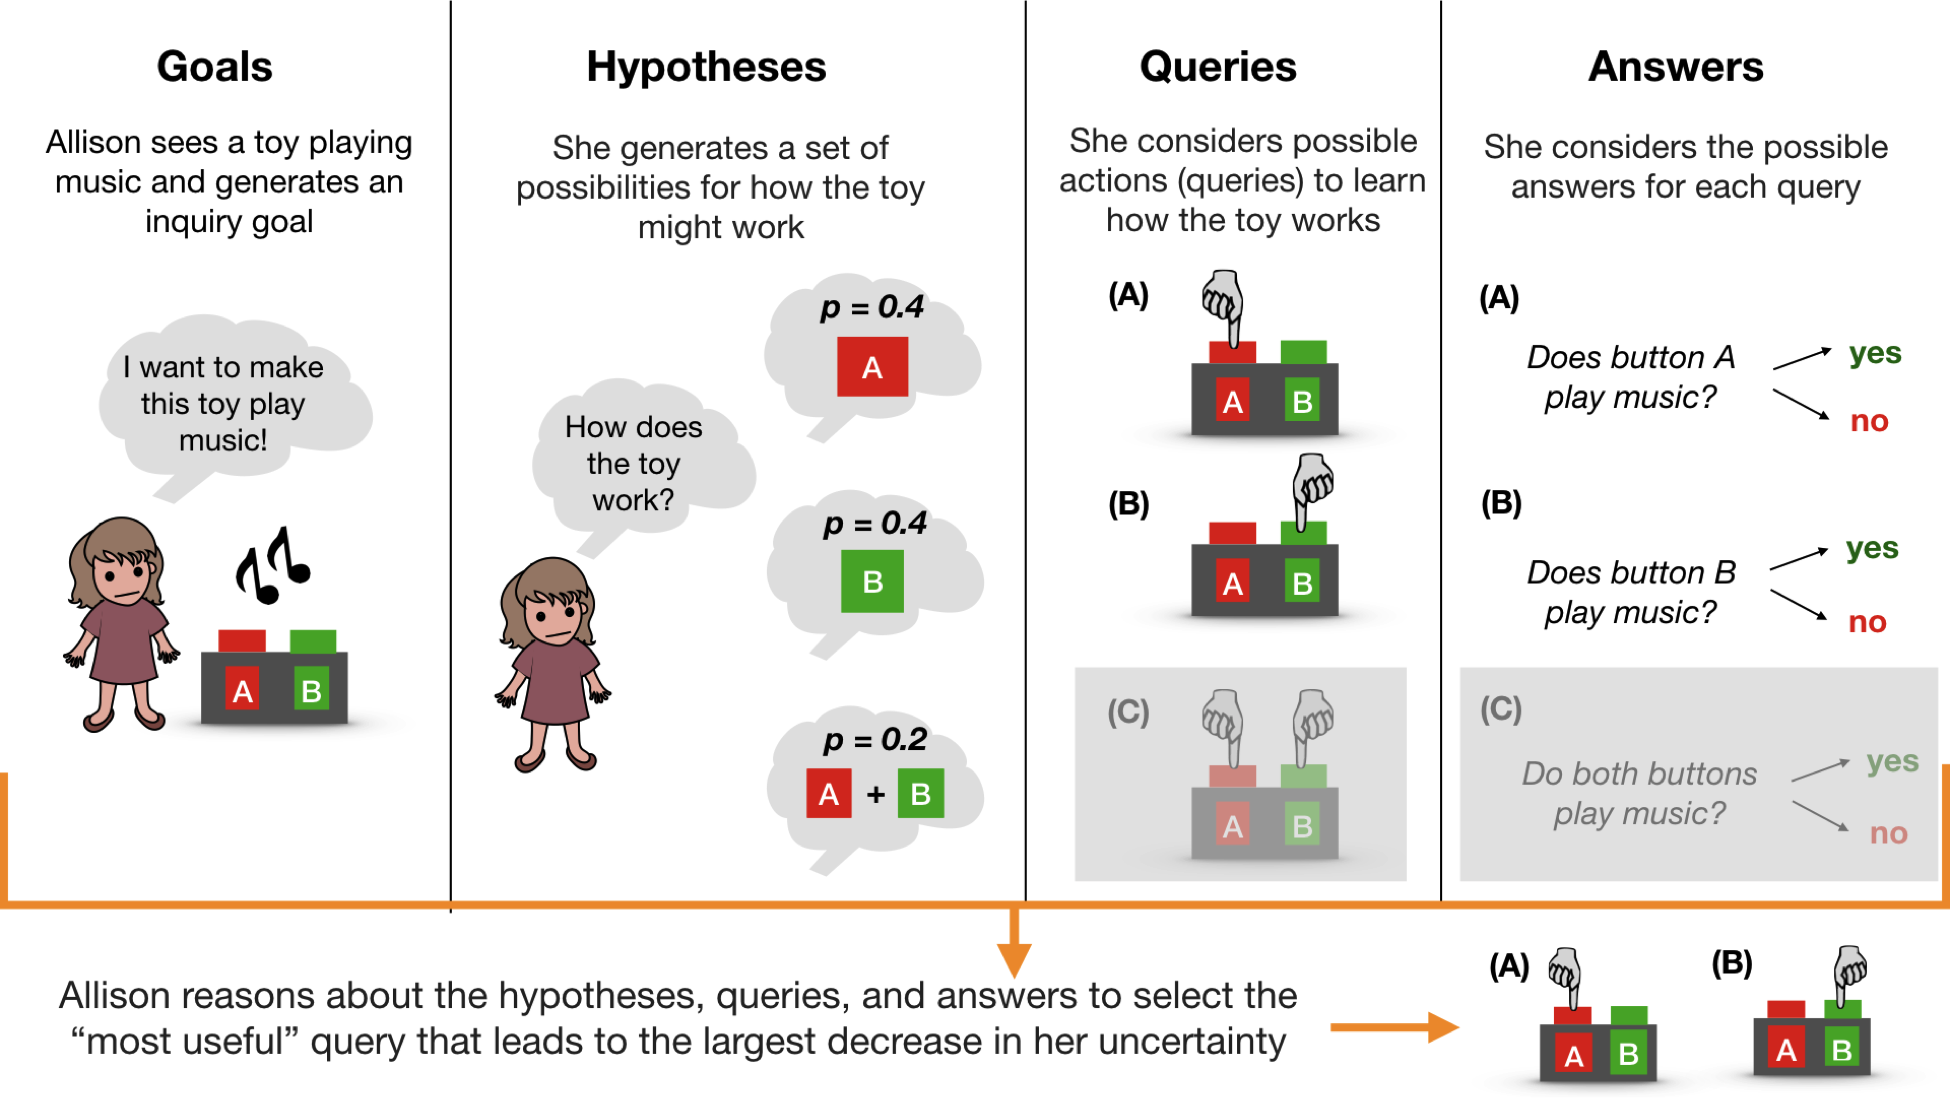
\includegraphics[width=1\linewidth]{macdonald_cada_files/figure-latex/unnamed-chunk-1-1} \caption{\textit{Schematic of an active causal learning context using the decomposition of Optimal Experiment Design. The learner generates an inquiry goal to learn how the toy works. She then considers hypotheses, including her subjective belief in each, placing stronger belief in the simpler, disjunctive hypotheses: only Button A or Button B. Next, she considers her possible queries (actions) and the potential outcomes if she took those actions. Together, these components quantify the expected usefulness of each action. If the learner chooses optimally, she picks the action that maximizes this expected utility. In this case, she chooses to press either Button A or B, but does not press both buttons since this action would produce confounded evidence and fail to reduce her uncertainty. See Part III in the text for mathematical details of the OED model.}}\label{fig:unnamed-chunk-1}
\end{figure}
\clearpage
}

Coenen, Nelson, and Gureckis (2017) provide a thorough review of the OED
framework and its links to human information seeking. They outline the
four critical parts of an OED model: (1) a set of hypotheses, (2) a set
of queries (i.e., actions) to learn about the hypotheses, (3) a way to
model the types of answers that each query could elicit, and (4) a way
to score each answer with respect to the learning goal. They also
highlight the importance of understanding learners' inquiry goals (what
do people want to learn?) for engaging OED-like reasoning. The critical
point is that without a clear learning goal, it becomes challenging to
instantiate the hypotheses, questions, and answers that a learner should
consider. In the rest of this section, I provide the mathematical
details of the OED approach as described in Coenen et al. (2017). The
goal is to provide a concrete foundation for the conceptual analysis of
how social learning contexts can influence different components of
active learning.

The OED model quantifies the \emph{expected utility} of different
information seeking actions. Formally, the set of queries is defined as
\(Q_1, Q_2,..., Q_n = \{Q\}\). The expected utility of each query
(\(EU(Q)\)) is a function of two factors: (1) the probability of
obtaining a specific answer \(P(a)\) weighted by (2) the usefulness of
that answer for achieving the learning goal \(U(a)\).

\[EU(Q) = \sum_{a\in q}{P(a)U(a)}\] \noindent
There are a variety of ways to define the usefulness function to score
each answer. An exhaustive review is beyond the scope of this paper (for
a detailed analysis of different approaches, see Nelson (2005)). One
standard method is to use \emph{information gain}, which is defined as
the change in the learner's overall uncertainty (difference in entoropy)
before and after receiving an answer.

\[U(a) = ent(H) - ent(H|a)\]

\noindent
Where \(ent(H)\) is defined using Shannon entropy\footnote{Shannon
  entropy is a measure of unpredictability or amount of uncertainty in
  the learner's probability distribution over hypotheses. Intuitively,
  higher entropy distributions are more uncertain and harder to predict.
  For example, if the learner believes that all hypotheses are equally
  likely, then they are in a state of high uncertainty/entropy. In
  contrast, if the learner firmly believes in one hypothesis, then
  uncertainty/entropy is low.} (MacKay, 2003), which provides a measure
of the overall amount of uncertainty in the learner's beliefs about the
candidate hypotheses.

\[ent(H) = -\sum_{a\in A}{P(h)log_2P(h)}\] \noindent
The conditional entropy computation is the same, but takes into account
the change in the learner's beliefs after seeing an answer.

\[ ent(H|a) = -\sum_{h\in H}{P(h|a)logP(h|a)} \] \noindent
To calculate the change in the learner's belief in a hypothesis
\(P(h|a)\), we use Bayes rule.

\[ P(h|a) = \frac{P(h)P(a|h)}{P(a)} \]

\noindent
If the researcher defines all these parts of the OED model (hypotheses,
questions, answers, and the usefulness function), then selecting the
optimal query is straightforward. The learner performs the expected
utility computation for each query in the set of possible queries and
picks the one that maximizes utility. In practice, the learner considers
each possible answer, scores the answer with the usefulness function,
and weights the score using the probability of getting that answer.

Before reviewing the behavioral evidence for OED-like reasoning in
adults and children, I will present a worked example of how to compute
the expected utility of a single query. The goal is to provide simple
calculations that illustrate how reasoning about hypotheses, questions,
and answers can lead to selecting useful actions. This example is
slightly modified from Nelson (2005).\footnote{In the
  \protect\hyperlink{app}{appendix}, I include example code for
  instantiating the OED calculations as functions in the R programming
  language.}

Imagine that you are a biologist, and you come across a new animal that
you think belongs to one of two species: \enquote{glom} or
\enquote{fizo.} You cannot directly query the category identity, but you
can gather information about the presence or absence of two features
(eats meat? or is nocturnal?) that you know from prior research are more
or less likely for each of the species. The following probabilities
summarise this prior knowledge:

\begin{itemize}
\tightlist
\item
  \(P(eatsMeat \mid glom) = 0.1\)\\
\item
  \(P(eatsMeat \mid fizo) = 0.9\)
\item
  \(P(nocturnal \mid glom) = 0.3\)\\
\item
  \(P(nocturnal \mid fizo) = 0.5\).
\end{itemize}

\noindent   You also know from previous research that the probability of
seeing a glom or a fizo in the wild is:

\begin{itemize}
\tightlist
\item
  \(P(glom) = 0.7\)
\item
  \(P(fizo) = 0.3\)
\end{itemize}

\noindent   Which feature should you test: eats meat? or sleeps at
night? Intuitively, it seems better to test whether the creature eats
meat because an answer to this question provides good evidence about
whether the animal is a fizo since \(P(eatsMeat \mid fizo) = 0.9\).
However, the OED computation allows the biologist to go beyond this
intuition and compute precisely how much better it is to ask the
\enquote{eats meat?} question. All the scientist has to do is pass her
knowledge about the hypotheses and features through the expected utility
computation.

Here are the steps of the OED computation for calculating the utility of
the \enquote{eats meat?} question. First, we use Bayes rule to calculate
how much our beliefs would change if we received a \enquote{yes} or a
\enquote{no} answer.\footnote{Note that the \(P(eatsMeat)\) term is
  computed by taking
  \(P(eatsMeat) = [P(eatsMeat \mid glom) \ times P(glom)] + [P(eatsMeat \mid fizo) \times P(fizo)] = (0.1 \times 0.7) + (0.9 \times 0.3) = 0.34\)}

\[ P(glom \mid eatsMeat) = \frac{P(eatsMeat \mid glom) \times P(glom)}{P(eatsMeat)} = \frac{0.1 \times 0.7}{0.34} = 0.21 \]

\noindent
Next, we calculate the uncertainty over the Species hypothesis before
doing any experiment. We do this by computing the prior entropy.

\[
\begin{aligned}
ent(Species) &= -\sum_{h\in H}{P(h) \times log_2P(h)} \\
 &= [-P(glom) \times log_2P(glom)]+[-P(fizo) \times log_2P(fizo)]\\
 &= [-(0.7 \times log_2(0.7)] + [-(0.3 \times log_2(0.3)]\\
 &= 0.8
\end{aligned}
\]

\noindent
To calculate information gain, we also need to compute our uncertainty
over hypotheses conditional on seeing each answer, or the posterior
entropy. First, for the \enquote{yes} answer:

\[
\begin{aligned}
ent(Species|eatsMeat = yes) &= -\sum_{a\in A}P(Species \mid eatsMeat = yes) \times log_2P(species \mid eatsMeat = yes) \\
&= [0.21 \times log_2(0.21)] + [0.79 \times log_2(0.79)]\\
&=  0.15
\end{aligned}
\]

\noindent
We use the difference between the prior and posterior entropy to compute
the utility of the \enquote{yes} answer.

\[
\begin{aligned}
U(a) &= ent(Species) - ent(Species \mid eatsMeat = yes)\\
&= 0.8 - 0.15 \\
&= 0.65
\end{aligned}
\]

\noindent
Next, we do the same process for the \enquote{no} answer. First, we
calculate the posterior entropy.

\[ 
\begin{aligned}
ent(Species|eatsMeat = no) &= -\sum_{a\in A}{P(Species \mid eatsMeat = no) \times log_2P(species \mid eatsMeat = no)}\\
&= [0.95 \times log_2(0.95)] + [0.04 \times log_2(0.04)]\\
&=  0.62
\end{aligned}
\]

\noindent
And use the difference between the prior and posterior entropy to
compute the utility of the \enquote{no} answer.

\[ 
\begin{aligned}
U(a) &= ent(Species) - ent(Species \mid eatsMeat = no)\\
&= 0.8 - 0.62 \\
&= 0.18
\end{aligned}
\]

\noindent
Finally, to get the overall information gain of the \enquote{eats meat}
\textbf{question}, we weight the utility of each answer by its prior
probability:

\[
\begin{aligned}
EU(Q = eatsMeat) &= \sum_{a\in A}{P(a)U(a)} \\
&= [P(eatsMeat = yes) \times U(eatsMeat = yes)] + \\& \qquad \qquad \qquad [P(eatsMeat = no) \times U(eatsMeat = no)]\\
&= [0.34 \times 0.65] + [0.66 \times log_2(0.15)]\\
&= 0.43
\end{aligned}
\]

If we perform the same steps to compute the expected utility of the
\enquote{sleeps at night?} question, we get
\(EU(Q = sleepsNight) = 0.026\). So if the biologist wants to maximize
her chances of gaining useful information, she should select the
\enquote{eats meat?} experiment since
\(EU(Q = eatsMeat) > EU(sleepsNight)\).

\afterpage{
\begin{figure}[H]
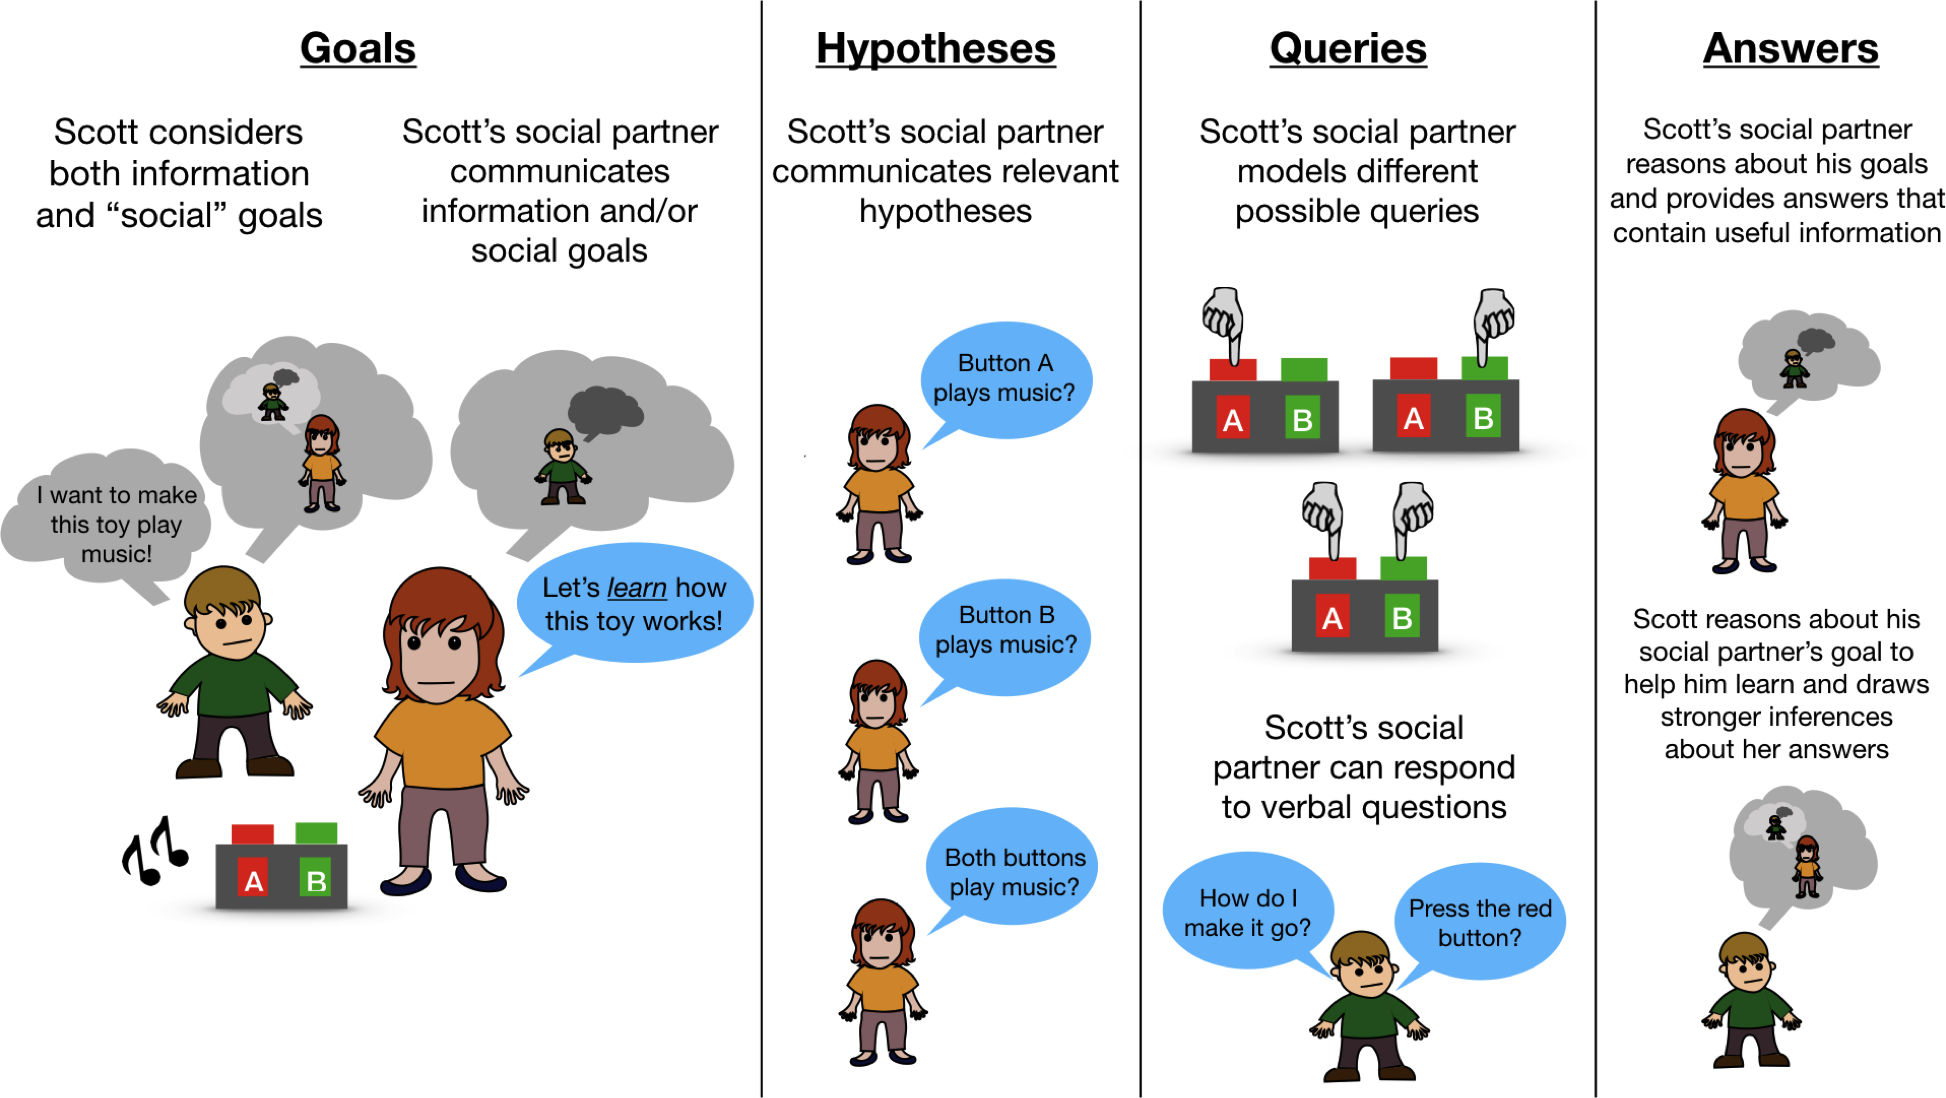
\includegraphics[width=1\linewidth]{macdonald_cada_files/figure-latex/unnamed-chunk-2-1} \caption{\textit{Schematic of an active word learning context using the decomposition of Optimal Experiment Design. Social input (hearing a novel word) triggers an inquiry goal. Then the learner considers potential hypotheses for the candidate word-object links, weighting each hypothesis by its prior probability. In this case, the learner thinks that the new word is less likely to refer to the familiar object BALL. Next, he considers possible queries (actions) and the potential outcomes of those actions. Note that in the word learning context, the child must direct queries towards a social partner, which provides the learner with more possible queries: both verbal (questions) and nonverbal (eye gaze; pointing). Note that the social partner must interpret the goal of the child's nonverbal queries. If the learner selects the action to maximize expected utility, then he would ask the most informative question, which removes all uncertainty for the meaning of 'dax' -- 'What's that called?' If he does select the relatively less informative action of asking about a single object, he would be unlikely to ask about the familiar object BALL since there is less information to be gained from this query based on his prior beliefs.}}\label{fig:unnamed-chunk-2}
\end{figure}
\clearpage
}

\subsubsection{Evidence of OED-like reasoning in human
behavior}\label{evidence-of-oed-like-reasoning-in-human-behavior}

A growing body of psychological research has used the OED framework as a
metaphor for active learning. The idea is that when people make
decisions, they are engaging in a similar process of evaluating the
\enquote{usefulness} of these different actions relative to some
learning goal. And, in turn, they select behaviors that maximize the
potential for gaining information. One of the significant successes of
the OED model is that it can be used to account for a wide range of
information seeking behaviors, including verbal question asking (Ruggeri
\& Lombrozo, 2015), planning interventions in causal learning tasks
(Cook, Goodman, \& Schulz, 2011), and decisions about where to look
during scene understanding (Najemnik \& Geisler, 2005).

One compelling demonstration of the OED metaphor for human behavior
comes from Nelson (2005) model of eye movements during novel concept
learning. The model combines Bayesian probabilistic learning, which
represents the learner's current knowledge as a probability distribution
over a concept, with an OED model of the usefulness of eye movements.
Here eye movements are modeled as a type of question-asking behavior
that gathers information about the target concept from the visual world.
Nelson (2005) found that participants' eye movements aligned with
predictions from the OED model. Specifically, participants changed the
dynamics of eye movements depending on how well they learned the target
concepts. For example, early in learning, when the concepts were
unfamiliar, the model predicted a broader, less efficient distribution
of fixations to all candidate features that could be used to categorize
the stimulus. However, after the model learned the target concepts, eye
movement patterns shifted, becoming more efficient and focusing on a
single stimulus dimension. This shift from exploratory to efficient eye
movements is exactly what adults did in the category learning task.

Recent developmental work has used OED models to test whether children
are capable of selecting efficient behaviors that maximize learning
goals. For example, Legare, Mills, Souza, Plummer, and Yasskin (2013)
used a modified question asking game where 4- to 6-year-old children saw
16 cards with a drawing of an animal on them. The animals varied along
several dimensions, including type, size, and pattern. Children could
ask the experimenter yes-no questions to figure out which animal card
was hidden in a box. Legare et al. (2013) coded questions as either
constraint-seeking (narrowing the set of possible cards by gathering
information about a particular dimension (e.g., \enquote{Is it red?}),
confirmatory (questions that provided redundant information), or
ineffective that did not provide any useful information (e.g.,
\enquote{Does it have a tail?}). All children produced a high proportion
of the more useful, constraint-seeking questions. Moreover, the number
of constraint-seeking questions was correlated with accuracy in guessing
the identity of the card hidden in the special box. Legare et al. (2013)
interpreted these results as evidence for OED-like reasoning in
children's question asking. Other work using the question-game finds
that children prefer to direct questions to someone who is knowledgeable
compared to someone who is inaccurate or ignorant, providing additional
support for the OED hypothesis (Mills, Legare, Bills, \& Mejias, 2010;
Mills, Legare, Grant, \& Landrum, 2011).

Another example of a direct link between OED models and children's
behavior comes from Cook et al. (2011) study of causal learning. They
showed preschoolers a device that played music when beads were placed on
top of it and manipulated the usefulness of different actions that
children could take to test the device. Half of the children saw
evidence that all types of beads could make the machine work, while the
other half learned that only specific types of beads (defined by color)
could make it go. Next, children could choose one of two sets of beads
to test the machine. In one set the beads were stuck together, in the
other, they could be separated. Children who learned that only some of
the beads worked were twice as likely to select the separable beads.
This finding suggests that children were reasoning about the amount of
information they could gain by choosing the detachable beads since this
choice would allow them to test each bead independently. In contrast,
the children who believed that all beads worked had less to gain by
picking the separable set. This result is compelling because it provides
evidence that children's were reasoning about a decision (separable
vs.~stuck together beads) that would influence a future opportunity to
generate useful information.

Although the OED approach has provided a formal account of seemingly
unconstrained information seeking behaviors, there are several ways in
which it falls short as an explanation of human self-directed learning.
Coenen et al. (2017) argue that OED models make several critical
assumptions about the learner and the learning task, including (1) the
hypotheses/questions/answers under consideration, (2) that people are
actually engaging in some expected utility computation in order to
maximize the goal of knowledge acquisition, and (3) that the learner has
sufficient cognitive capacities to carry out the calculations.

In the next section, I argue that limitations of the OED approach can be
productively reconstrued as opportunities for understanding how learning
from other people can scaffold active learning. I focus on integrating
research and theory on social learning with five key components of the
OED model: inquiry goals, hypotheses, questions, answers, and stopping
rules. The key insight is that learning from more knowledgeable others
provides the building blocks for children to engage in productive
self-directed learning.

\hypertarget{p4}{\section{Part IV: Active learning within social
contexts}\label{p4}}

Why should social contexts shape active learning? First, children do not
re-invent knowledge of the world, and while they can learn a tremendous
amount from their behaviors, much of their generalization and
abstraction is shaped by input from other people. Moreover, social
learning can sometimes be the only way to learn something. And children
are often surrounded by parents, other adults, and older peers -- all of
whom may know more about the world than they do, creating contexts where
the opportunity for social learning is ubiquitous.

Second, there is a body of empirical work showing that active learning
can be biased and ineffective in systematic ways. For example, work by
Klahr and Nigam (2004) showed that elementary school-aged children were
less effective at discovering the principles of well-controlled
experiments from their self-directed learning, but were capable of
learning these principles from direct instruction. D. B. Markant and
Gureckis (2014) showed that active exploration provided no benefit over
passive input in category learning when there was a mismatch between the
target concept and adults' prior hypotheses going into the learning
task. And McCormack et al. (2016) found that 6-7 year-olds showed no
benefit from active interventions on a causal system compared to
observing another person perform the interventions.

In a comprehensive review of the self-directed learning literature,
Gureckis and Markant (2012) point out that the quality of active
exploration is linked to aspects of the learner's understanding of the
task: if the representation is weak, then self-directed learning will be
biased and ineffective. Coenen et al. (2017) go a step further and
propose specific challenges for research on active learning. Here is a
sampling of those open questions that are most relevant to my argument:

\begin{itemize}
\tightlist
\item
  What triggers inquiry behaviors in the first place?
\item
  How do people construct a set of hypotheses?
\item
  How do people generate a set of queries?
\item
  What makes a \enquote{good} answer?
\item
  How do people generate and weight possible answers to their queries?
\item
  How does learning from answers affect query selection and belief
  change?
\end{itemize}

\noindent
In the next section, I propose that social learning theories and
findings have something to say in addressing these challenges. I use the
OED model outlined in Coenen et al. (2017) as a starting point for
defining inquiry behavior and use it to integrate the social and active
learning accounts. The benefit of this formalization is that it makes
the different components of active learning explicit, making salient the
aspects that might be particularly challenging for young learners with
limited cognitive resources. I propose that we can reconstrue the
\enquote{limitations} of the OED account as opportunities for
understanding the role of other people in children's active learning. In
each sub-section, I first define the challenge of active learning. Then,
I discuss how social contexts could address each challenge while
highlighting prior research that connects the active and social learning
accounts.

\subsection{Goals}\label{goals}

An inquiry goal refers to the underlying motivation for people's
information seeking behaviors. Often this is defined as a search for the
correct hypothesis amongst a set of candidate hypotheses. Intuitively,
an inquiry goal is what drives people to learn. Some examples of
plausible inquiry goals include:

\begin{itemize}
\tightlist
\item
  Is this person a reliable source of information? (selective learning)
\item
  What is this speaker referring to? (word learning)
\item
  What types of objects are called \enquote{daxes}? (category learning)
\item
  How does this toy work? (causal learning)
\item
  Where should I look next? (allocation of visual attention)
\end{itemize}

\noindent
Without an explicit inquiry goal, it becomes difficult for an active
learner to compare the utility of different behaviors since the learner
cannot evaluate how an action will lead to learning progress. Coenen et
al. (2017) illustrate this point by pointing out how researchers often
go to great lengths to communicate the specific inquiry goal of an
experimental task, saying:

\begin{quote}
The importance of such goals is made clear by the fact that in
experiments designed to evaluate OED principles, participants are
usually instructed on the goal of a task and are often incentivized by
some monetary reward tied to achieving participants that goal.
Similarly, in developmental studies, children are often explicitly asked
to answer certain questions, solve a particular problem, or choose
between a set of actions. (p.~32-33)
\end{quote}

\noindent
Characterizing children's goals becomes critical for evaluating the role
of self-directed behavior in cognitive development. However, this is not
easy since children could be considering a wide range of goals at any
moment and there is no guarantee that learning progress is one of them.
In fact, one line of theorizing about the OED hypothesis as a model of
human inquiry argues that we should only expect to see effective
information seeking in contexts where there are precise tasks and
learning goals. For example, when a parent gives their child a new toy
with several buttons on it and says, \enquote{Let's figure out how this
toy works!} In this case, it becomes possible to ask whether the child
approaches the task efficiently by selecting actions that provide useful
information about the toy's causal structure.

This example illustrates how children's interactions with other people
could play a role in triggering inquiry behavior. Both adults and older
peers can construct contexts with clear learning goals to support
children's information seeking. This connection draws on influential
ideas in cognitive development that frame social learning as a form of
scaffolding (Zone of Proximal Development (Vygotsky, 1987), Guided
Participation (Rogoff et al., 1993), and Guided Play (Weisberg,
Hirsh-Pasek, \& Golinkoff, 2013)). Under these accounts, adults place
children in contexts that present something new to be learned but
importantly contain learning goals that are achievable given children's
current capabilities.

For example, Weisberg et al. (2013) define \enquote{guided play} as an
intermediate learning context, falling between unstructured free play
and constrained direct instruction. Unfortunately, the boundaries
between these contexts are underspecified and challenging to define, but
the critical dimension is the level of control that the adult exerts
over the activity. They present the following example to illustrate the
key difference between guided play and direct instruction.

\begin{quote}
For example, a teacher with the goal of teaching new vocabulary words
could take a direct instruction approach, by telling children the
meanings of the new words they encounter in a storybook or by showing
examples: \enquote{This is a helmet. A helmet goes on your head to stop
your head from getting hurt if you fall off your bike.} Or, she could
take a guided-play approach, introducing the new words in the context of
a child's play episode while encouraging children to think broadly about
the word's meaning: ``She's got a helmet on while riding her bike. What
do you think would happen if she fell off her bike and wasn't wearing
her helmet? (p.~106)
\end{quote}

\noindent
While these contexts appear quite similar, the key difference is whether
the child initiated the activity. In free play, the child drives the
interaction; whereas, in direct instruction, the more knowledgeable
person explicitly tells the learner what to do, asks questions, and
demonstrates new concepts. Weisberg et al. (2013) hypothesize that the
guided play context provides the right combination of structure with
opportunity for exploration, leading to better learning outcomes.

One less-emphasized feature of the Guided Play proposal is the adult
initializing a clear learning goal. In the previous example, without the
presence of a social partner, it is unclear what goals the child would
pursue when playing with a storybook. However, the presence of an adult
who has knowledge of the names of objects in the book and has the goal
to teach changes the potential for the child to engage in
information-seeking. We can frame this discussion in the terms the OED
hypothesis, and say that one critical function of other people is to
create contexts where there is something to learn. These settings
trigger inquiry goals, which, in turn, sets the stage for children to
reason about the actions could support learning (e.g., what question to
ask or what object to point out).

In addition to communicating inquiry goals, the mere presence of others
can affects children's tendency to detect whether they understand
something. This capacity for explicitly reasoning about one's
uncertainty is a component of metacognition and has been the focus of a
great deal of developmental research (see Lyons and Ghetti (2010) for a
review). The upshot of this work is that while children might be capable
of showing behaviors that are sensitive to uncertainty (e.g.,
selectively exploring an object with ambiguous causal structure), the
ability to have explicit access to the underlying representation of
uncertainty is slower develop.

There are striking experimental demonstrations of children's failure to
monitor their uncertainty. For example, Markman (1979) had elementary
school aged children read paragraphs with inconsistent information
(e.g., \enquote{fish can't see without light, and there's no light at
the bottom of the ocean, but some fish at the bottom of the ocean only
know their food by its color.}). After reading the paragraph, children
answered 10 questions that gave them the opportunity to ask for
clarification about the inconsistency. Overall, participants were not
great at the task, as Markman (1979) put it, \enquote{even highly
motivated children} were unable to detect inconsistencies in the
incoming information. However, if children were provided with a warning
or a challenge to find a problem with the essay, they generated more
questions, demonstrating higher rates of uncertainty monitoring.

While not discussed in these terms, Markman (1979) \enquote{warning}
manipulation can be reconstrued as an intervention of the social context
on children's expectations. That is, children might approach social
interactions with a default expectation that adults will provide
complete information.\footnote{See the work on children's pedagogical
  sampling assumptions reviewed in \protect\hyperlink{p1}{Part I}and the
  discussion of Answers later in this section for additional evidence
  that children's default assumption is that others will be helpful
  during communicative interaction.} But when the social context shifts
these expections, then children are more likely to monitor the input for
inconsistency, and in turn, more likely to generate inquiry goals.

Converging evidence comes a study by Kim, Paulus, Sodian, and Proust
(2016)\enquote{s where they measured 3- to 4-year-olds} uncertainty
monitoring in contexts where children either did or did not expect to
communicate with another person. In the task, Children were either
knowledgeable or ignorant about which toys an experimenter hid in a box.
In the \enquote{informing} condition, children had to tell another
person about the contents of the box, but they were given the
opportunity to \enquote{opt-out} of responding if they were unsure
(\enquote{Max wants to know what's inside the box. Can you help him? If
you do not want to tell him, it's okay. I can tell him.}). In the
\enquote{explicit} condition, children just reported on their
uncertainty. Interestingly, the children who had the potential to inform
another person showed higher rates of uncertainty monitoring, opting-out
of more often when they did not know what was inside the box. Similar to
the Markman (1979) finding, the social context shifted children's
expectations, making them more likely to detect lack of knowledge. These
results also dovetail with work showing that the process of generating
explanations for other people (and for ourselves) is a powerful way to
reveal inconsistencies in our understanding (Lombrozo, 2006).

Another interesting link between social learning research and children's
goals during learning comes from work exploring how input shapes
implicit theories of intelligence (Dweck \& Leggett, 1988). Implicit
theories of intelligence refer to children's internal working models of
the world and provide general frameworks for processing information and
generating predictions about behavior. Dweck and Leggett (1988) propose
a cognitive model where holding different implicit theories of
intelligence leads children to adopt different goal orientations, which
manifest in different choice behavior during learning. For example, if a
child holds the belief that intelligence is malleable (an incremental
theory), they will want to increase competence (select a learning goal)
and therefore be more likely to choose tasks that facilitate learning.

Empirical work shows that social partners can directly intervene on
children's learning vs.~performance goals. For example, Elliott and
Dweck (1988) directly manipulated elementary school-aged children's
goals by presenting them with a choice between one of two tasks
described in the following ways:

\begin{itemize}
\tightlist
\item
  \emph{Performance task}. In this box we have problems of different
  levels. Some are hard, some are easier. If you pick this box, although
  you won't learn new things, it will really show me what kids can do.
\item
  \emph{Learning task}. If you pick the task in this box, you'll
  probably learn a lot of new things. But you'll probably make a bunch
  of mistakes, get a little confused, maybe feel a little dumb at times
  --- but eventually you'll learn some useful things.
\end{itemize}

\noindent
Elliott and Dweck (1988) found that when children oriented towards the
learning goal tended to choose the more difficult \enquote{learning}
task even though they were likely to make mistakes and risk looking
incompetent. In another study, Dweck and Leggett (1988) showed that
children who already held performance goals viewed effort on a task as
an index of ability, whereas children with learning goals viewed effort
as a means for improvement. Moreover, both lab-based experiments and
observational work provide evidence that the language adults choose to
use when praising children influences their implicit theories (Cimpian,
Arce, Markman, \& Dweck, 2007; Gunderson et al., 2013).

Taken together, the research on implicit theories suggests another way
social contexts can trigger inquiry goals. The Elliott and Dweck (1988)
finding -- that children who were oriented toward learning goals
selected more challenging tasks -- directly maps onto behaviors that the
OED framework aims to characterize. That is, the goal manipulation is an
example of the social context pushing children towards an inquiry goal,
which encourages behaviors that make progress towards learning. This
process of triggering inquiry goals is an explicit pre-requisite in the
OED model.

The social context can also introduce \enquote{social} goals that
directly influence children's information seeking. The core OED
framework only includes the goal of information seeking such that the
utility of behavior is based solely on how actions lead to changes in
the uncertainty about hypotheses. However, other empirical and modeling
work has expanded on the basic information-seeking account to include
\emph{situation-specific utility functions} that include goals such as
saving time, money, or cognitive resources. For example, Meder and
Nelson (2012) designed a series of experiments where \enquote{pure}
information seeking goals (e.g., maximizing accuracy) were placed at
odds with the reward structure of the task. The critical manipulation
was including asymmetric rewards for correct and incorrect
categorization decisions in a binary classification task. Asymmetric
rewards forced the learner to choose the less likely category to earn
the highest reward (i.e., they must be willing to forego the goal of
being accurate and make mistakes to get the highest score). When these
goals were put in conflict, participants' behavior was mixed.
Participants only reduced their preference for information seeking and
improving accuracy when the asymmetric reward structure was made
explicit via task instructions. However, Meder and Nelson (2012)
speculate that people were able to consider goals other than pure
information gain or reward maximization, taking the results as evidence
for the need to consider additional factors when trying to understand
the behaviors that people think are most useful.

One compelling aspect of social contexts is that they engage a process
of psychological reasoning about others' mental lives. And once the
learner starts thinking about the other person, they could begin to
consider an additional set of \enquote{social} goals that may conflict
with or support their learning goals. Consider the schematic
active-social learning context in Figure 3. If Scott is worried about
whether his social partner thinks he is smart, then he might prioritize
actions that minimize the chance of making a mistake and perhaps not
even attempt to make the toy work. Scott might seek out easy tasks to
demonstrate his competence at the expense of choosing actions that help
him learn about the world. On the other hand, Scott's social partner
could explicitly communicate the learning goal using natural language,
e.g., \enquote{Let's learn how this toy works!} This dovetails with the
experimental results in Elliott and Dweck (1988) reviewed above.

Recent work by E. J. Yoon, Tessler, and Frank (2017) has aimed to
include a broader range of goals in models of pragmatic communication.
Specifically, they are interested in the topic of polite speech (e.g.,
people using indirect language such as \enquote{I don't think that dress
looks phenomenal on you} as opposed to \enquote{It looks terrible}) as a
tradeoff between information and social goals. In their model, speakers
reason about their actions concerning the information goal -- to
communicate information faithfully with as little effort as possible --
and a social goal -- to avoid harm to one's own or another's self-image.
E. J. Yoon et al. (2017) build on the Rational Speech Act (RSA)
framework for pragmatic reasoning\footnote{RSA models language
  comprehension and production as, \enquote{a process of recursive
  reasoning about what speakers would have said, given a set of
  communicative goals} (p.819).} (Goodman \& Frank, 2016). We can draw a
direct connection between the polite RSA model and the OED account. Both
assume that people produce actions to maximize utility, but the polite
RSA expands the utility function, modeling overall utility of an
utterance as a weighted combination of social and informational goals.

An intriguing possibility for future research would be to adapt the
utility-theoretic approach used by E. J. Yoon et al. (2017) to
children's information seeking behaviors in social contexts. We can also
connect these ideas to the effects of task framing (performance
vs.~learning oriented) on children's decisions to try more challenging
tasks. The presence of another person could be modeled as an increase in
the weight that children place on maximizing social goals, leading
children to select easier tasks where they can appear competent. This is
an interesting extension of the goal-orienting account reviewed above in
that it frames these effects as a mixture of goals as opposed to the
social context triggering either a performance or a learning goal.

One important gap in the current understanding of children's inquiry
goals is a reasonable estimate of how often children participate in
contexts with clear learning goals in their daily lives. Moreover, we do
not yet have a theory of the kind of settings that would lead children
to generate inquiry goals. However, work on rates of \emph{Guided
participation} across cultures provides an interesting counter-example
(Rogoff et al., 1993). @Rogoff et al. (1993) coded the amount of
\enquote{caregiver orienting} behavior present in parent-child
interactions with their 12- to 24-month-old infants across four
different cultural communities (a Mayan Indian town in Guatemala, a
middle-class urban group in the United States, a tribal village in
India, and a middle-class urban neighborhood in Turkey) that varied
along the dimensions of how separated children were from adult
activities and whether formal schooling was emphasized. Caregiver
orienting was defined as,

\begin{quote}
Caregiver orients child involved introducing new information or
structure to the child (at any point in the episode) regarding the
overall goals or a key part of the event or what was expected in the
situation. Orienting framed a major goal, not just specific little
directives for particular actions. (p.~43)
\end{quote}

\noindent
Rogoff et al. (1993) found that parents in all four communities produced
high rates of structuring and orienting behaviors (with the lowest rate
of structuring being 81\% of play episodes). Thus, when placed in a
structured activity, adults make sure children are aware of the goal
(e.g., learning the function of the novel toy). However, the communities
differed in how often children were directly involved with adult
activities in day-to-day life, with the children raised in rural
villages often having early access to adult economic and social events.
An interesting open question is whether older peers and adults need to
be directly engaging with the child to trigger inquiry goals. Perhaps
increased access to observing adult goal-directed behaviors can
facilitate learning goals. For example, it could be generating lots
inquiry goals would be a byproduct of seeing lots of adult activities
(e.g., cooking, shopping, working) that they do not understand.

In sum, understanding children's goals represent a critical step in
characterizing the relative contribution active learning to cognitive
development. Social contexts have the power to trigger inquiry goals,
but also can introduce alternative social goals that might be at odds
with children's decisions about what to learn. One important direction
for future research is to map the space of children's goals during
everyday learning contexts. It would be useful to know how much of
children's daily activities involve settings where there is a clear
learning goal either generated independently by the child or
communicated by older peers and adults. It would also be useful to know
how the distribution of these goals change as a function of development,
especially as children enter school and across different cultural
contexts where children have differential access to structured (e.g.,
lessons and sports) vs.~unstructured activies (e.g., free play). Moving
beyond the lab-based studies of OED-like reasoning is no easy task and
will require leveraging recent advances in large-scale observational
data collection about children's daily experiences.

\afterpage{
\begin{figure}[H]
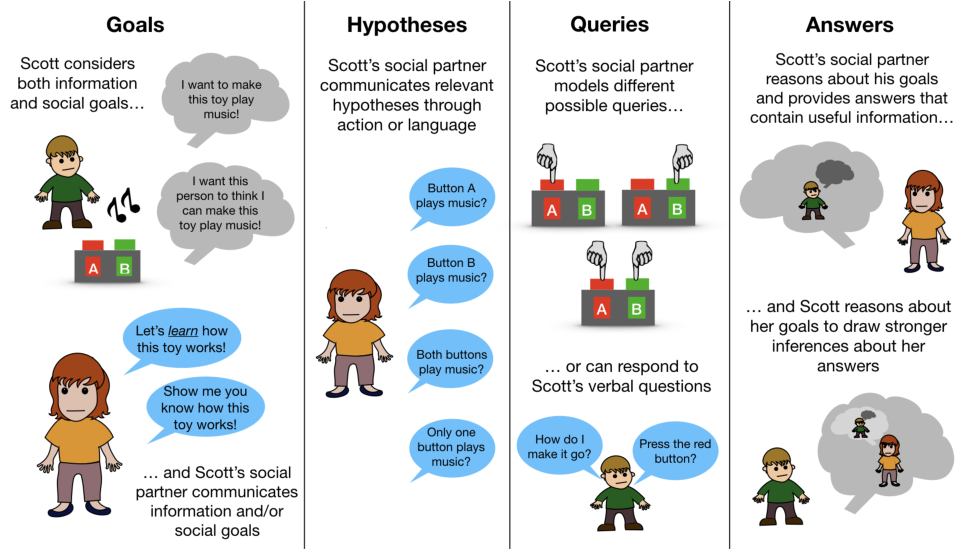
\includegraphics[width=1\linewidth]{macdonald_cada_files/figure-latex/unnamed-chunk-3-1} \caption{\textit{Schematic of active learning within a social context. Each panel shows how social information could influence a different component of the active learning process. These social effects occur in-the-moment of learning or over developmental time. Also, the cause of the social effect varies from the mere presence of another person to triggering a sophisticated psychological reasoning process about others' goal-directed behaviors. Note that the panels correspond to the different sub-sections in Part IV of the text.}}\label{fig:unnamed-chunk-3}
\end{figure}
\clearpage
}

\subsection{Hypotheses}\label{hypotheses}

After establishing learning goal, the next component of inquiry is
deciding what hypotheses the learner should consider. Intuitively, a
hypothesis is a candidate explanation about how the world works. For
example, consider the schematic learning contexts shown in Figures 1 and
2. In the casual context, the hypotheses for how the toy works could
include: (1) Button A, (2) Button B, (3) Buttons A and B simultaneously.
In the word learning context, the child might think the new word
\enquote{dax} means: (1) dax = object A, (2) dax = object B, or (3) dax
= object C.\footnote{Note that this hypothesis space is simplified since
  it only considers the possibility of one-to-one word-object mappings.}

The set of hypotheses under consideration is critical for effective
self-directed learning. The usefulness function -- expected information
gain -- outlined in \protect\hyperlink{p3}{Part III} works by comparing
the learner's uncertainty over hypotheses before and after she chooses
an action. Without knowing what is in the hypothesis space, it becomes
challenging to figure out the best choice for reducing uncertainty. Put
another way; the OED framework does not readily deal with situations
where learners might have to consider a large space of hypotheses, might
hold the wrong hypotheses, or might perform actions without considering
any hypotheses at all. This is an especially important challenge for
developmental accounts that draw on OED principles since these scenarios
seem quite plausible for young learners.

However, a critical function of social learning contexts is to provide a
clear set of possible explanations for the actual state of the world.
That is, adults and older peers, who might have access to the correct
hypothesis, can restrict children's hypotheses to guide their
information seeking. This effect of social context parallels the
discussion of goals reviewed in the previous section.

One relevant case study comes from work on children's early word
learning. The learning challenge is that even the simplest of words,
concrete nouns, are often used in complex contexts with multiple
possible referents, which in turn have many conceptually natural
properties that a speaker could talk about. This ambiguity creates the
potential for an (in principle) unlimited amount of hypotheses that
children could consider when trying to figure out the meaning a novel
word. Remarkably, word learning proceeds despite this massive
uncertainty, with estimates of adult vocabularies ranging from 50,000 to
100,000 distinct lexical concepts (P. Bloom, 2002).

It does not seem plausible for children to entertain all hypotheses
about possible word-object links. But which ones should they consider?
One proposed solution is that word learners only consider a single
word-object link at a time (Medina, Snedeker, Trueswell, \& Gleitman,
2011; Trueswell, Medina, Hafri, \& Gleitman, 2013). Under this account,
the child makes an initial guess about the word meaning, and then only
stores that word-object link until she receives sufficient evidence that
her initial hypothesis was incorrect. If she does see enough
counter-evidence, then she will switch to a new, single hypothesis that
better matches the statistics in the input.\footnote{This
  \enquote{propose-but-verify} account parallels work by E. Bonawitz,
  Denison, Gopnik, and Griffiths (2014) in the domain of causal
  learning, which suggests that a \enquote{Win-Stay, Lose-Sample}
  algorithm (inspired by efficient sampling procedures in computer
  science) provides a better explanation of children's hypothesis
  testing behaviors compared to an algorithm that enumerates the entire
  hypothesis space.} However, another influential account of early word
learning, inspired by basic associative learning principles, argues that
word learners store more than a single hypothesis. Under this theory,
children's hypothesis spaces are reduced gradually via the aggregation
of word-object co-occurrence statistics across multiple labeling events
(Siskind, 1996; C. Yu \& Smith, 2012b). Support for this account comes
from experimental work showing that both adults and young infants can
use word-object co-occurrence statistics to learn word meaning from
individually ambiguous naming events (Smith \& Yu, 2008). Moreover,
adults show evidence of being able to recall multiple word-object links
from an initial naming event (Yurovsky \& Frank, 2015).

The critical difference between these proposals is how much information
learners store in their hypothesis space. And understanding the nature
of these hypotheses is essential for evaluating children's ability to
seek information. Some of our own work provides evidence that the social
context can modulate the content of the learner's hypothesis space
(MacDonald, Yurovsky, \& Frank, 2017). Inspired by ideas from
Social-pragmatic theories of language acquisition that emphasize the
importance of social cues for word learning (P. Bloom, 2002; E. V.
Clark, 2009; Hollich et al., 2000), we showed adults a series of word
learning contexts that varied in ambiguity depending on whether there
was a useful social cue to reference present (i.e., a gaze cue). We then
measured learners' memory for alternative word-object links at different
levels of attention and memory demands. Learners flexibly responded to
the amount of ambiguity in the input, and as uncertainty increased, they
tended to store more word-object hypotheses. Moreover, we found that
learners stored representations with different levels of fidelity as a
function of the reliability of the social cue and despite having the
same amount of time to explore the objects during the initial labeling
event.

These results provide evidence that the content of learners' hypothesis
spaces changed as a function of social information. Further suppport for
this idea comes from experimental work showing that even children as
young as 16 months prefer to map novel words to objects that are the
target of a speaker's gaze and not their own (D. A. Baldwin, 1993), and
analyses of naturalistic parent-child labeling events shows that young
learners tended to retain labels accompanied by clear referential cues,
which served to make a single object dominant in the visual field (C. Yu
\& Smith, 2012a). One important direction for future research is to
measure the full causal pathway from variation in social information
through children's hypothesis spaces to their information seeking
behaviors. For example, it would be interesting to know whether
learners' subsequent questions or decisions about where to allocate
attention would be affected by the social context in which they were
first exposed to a new word.

A second case study that illustrates the importance of considering young
learner's hypothesis spaces comes from work by Lucas, Bridgers,
Griffiths, and Gopnik (2014) where they compared children and adult's
capacity for learning different kinds of causal structures. In the task,
participants saw a series of events that consisted of a training phase
where an experimenter placed objects on a box that either played or did
not play music. The participant's goal was to learn which objects, or
combination of objects, made the box work. In the disjunctive condition,
only single objects (A or C, but not A) made the toy play music. In the
conjunctive condition, only the combination of two different objects (A
and C) would make the toy play music. After seeing several
demonstrations, both children and adults were tested on ambiguous events
where they could either infer a disjunctive or conjunctive causal
relationship. Lucas et al. (2014) found that only children showed
evidence of learning the conjunctive relationship, even if the evidence
favored this interpretation. The authors speculate that adults were more
biased towards the disjunctive hypothesis since it is more common in
everyday experience; whereas children's prior beliefs are more diffuse,
leading them to be more sensitive to evidence in favor of the
conjunctive hypothesis.\footnote{Figure 1 illustrates a version of the
  active causal learning scenario. In this case, the learner believes
  that pressing both buttons to activate the toy is a less likely
  hypothesis. As a result, the query to test the conjunctive hypothesis
  \enquote{press both buttons} becomes less useful for gaining
  information since it would produce confounded evidence concerning her
  other, disjunctive hypotheses.}

Why should these findings matter for active learning? A key prediction
of the OED account is that learners will select behaviors that maximally
reduce uncertainty in their beliefs, which is often formalized as the
difference in entropy between the prior and posterior probability
distributions over hypotheses (i.e., \(P(h|a) = ent(H) - ent(H|a)\)).
Thus, the content of the hypothesis space and the uncertainty over each
hypothesis plays a direct role in evaluating the relative usefulness of
different actions. Moreover, features of the social context could bias
the content of children's hypothesis space. For example, Lucas et al.
(2014) suggest that,

\begin{quote}
Most of the time, adults do not need to dramatically change their
beliefs or abandon their hypotheses for dramatically different ones.
Indeed, doing so would be a liability: adults are expected to make
accurate predictions and good decisions, not bold inductive leaps.
Adults are also unlikely to have caregivers to correct their errors and
save them from poor choices. (p.~295)
\end{quote}

\noindent
This proposal makes a testable prediction: that contexts in which
learners \enquote{feel} safe to make mistakes would lead children to
consider and test a broader range of hypotheses. Another effect of the
social context highlighted in Lucas et al. (2014)'s study is that the
experimenters scaffolded children and adults consideration of the
disjunctive and conjunctive hypotheses. That is, their actions
constrained the hypothesis space to isolate learning and information
seeking effects. The \enquote{Hypotheses} panel of Figure 3 presents a
schematic illustration of this social context effect. Similar to the
research on goals, the majority of the work on hypotheses has focused on
lab-based studies. Thus, it is an open question as to how much of role
adults play in communicating relevant hypotheses during everyday
learning.

A final case study comes from research on children's conceptual (Gelman,
2009). Conceptual change is a \enquote{radical} reconstruction of an
intuitive theory about how the world works. For example, elementary
school-aged children tend to hold a mixture of beliefs about the shape
of the earth (Vosniadou \& Brewer, 1992). These theories range from a
flat earth theory that matches children's everyday perceptual
experiences (i.e., walking on flat ground) to the adult-like, sphere
model, which reflects the actual state of the world. Interestingly, some
children hold intermediate beliefs such as a dual-earth theory where
there are two earths: \enquote{a round one which is up in the sky and a
flat one where people live} (p.~550). The fact that some children
entertain a dual-earth theory suggests that they are actively
integrating their initial theory with the information they get from
other people who already have the correct, sphere theory. And for
children to hold the sphere model, they must have learned it from social
input.

There is also experimental evidence for the importance of social input
in children's reasoning about biological concepts. For example, the
concept of \enquote{alive} takes years to fully develop, with younger
children (under 10 years of age) often claiming that only animals, and
not plants, are alive. Opfer and Siegler (2004) tested the hypothesis
that evidence of goal-directed movement is critical for children's
extension of the \enquote{alive} concept. In their study, 5-year-olds'
were trained in different ways to think about the concept of a
\enquote{living thing} and then asked whether they believed that plants
were alive. Children either learned that plants were capable of
goal-directed movement (e.g., \enquote{The house plant is growing this
way. It needs the sunlight over here.}), that plants were capable of
growth, or that plants need water to survive. Children in the
goal-directed movement condition showed the most significant theory
revision, saying plants were also living things more consistently on a
post-intervention categorization task.

Additional evidence comes from research on the links between language
experience and performance on various cognitive tasks. For example,
empirical work shows that deaf children without access to a natural
language perform worse on Theory of Mind tasks (Peterson \& Siegal,
2000); that Korean speakers perform better than English speakers on
tasks that require categorizing based on tight vs.~loose distinctions,
which are lexicalized in Korean (McDonough, Choi, \& Mandler, 2003); and
that exposure to a first language reduces infants' capacity to detect
non-native phonetic contrasts (Maurer \& Werker, 2014).

Together, the findings reviewed in this section illustrate several
points for the active-social learning account. First, the set of
hypotheses that children consider are likely to be quite different from
adults (and possibly different from what the experimenter thinks the
child is considering). Second, children generate hypotheses using a
mixture of prior knowledge, expectations about the task, and social
input. There are (at least) two timescales through which social learning
can shape hypotheses. An in-the-moment timescale where others' behavior
constrains hypotheses for the current task -- for example, referential
gaze indicating candidate word-object mappings, or an adult suggesting a
disjunctive (one-block) vs.~a conjunctive (two-block) theory for how to
make a toy work. And a developmental timescale where prior interactions
with other people and cultural learning modify the hypotheses that
children bring to the learning task (e.g., the conceptual change and
language effects reviewed above).\footnote{We could make a further
  distinction between the developmental and the cultural timescales,
  where developmental refers to information acquired from interactions
  with others in the child's lifetime (e.g., disjunctive causal
  structures are more likely to occur in the world) and cultural refers
  to information that has accumulated throughout human evoluationary
  history (e.g., access to natural language or concepts such as the
  spherecial earth.)}

\subsection{Questions}\label{questions}

Queries in the OED framework refer to the experiments that a scientist
could conduct to gather information about their hypotheses. Queries in
human information seeking can refer to a variety of actions, including
verbal questions, pushing a button to figure out how a toy works, and
decisions about where to look. In fact, the capacity to provide general
principles that explain such a broad range of behaviors is one of the
strengths of the OED account.

The challenge for the young learner is to discover what behaviors are
available and of those actions which might be particularly useful for
gathering information. In this section, I illustrate how the social
learning context provides valuable input to this learning process via
demonstrations of the range of actions that learners could take to
gather information. I suggest that this process unfolds by children
imitating and by adults' modeling useful information seeking behaviors.

It seems obvious that children would look to older peers or adults to
learn what actions are possible and useful. However, a large body of
empirical work suggests that even young infants will not imitate every
action that they see. Instead, children show evidence of
\enquote{rational imitation} and will look for cues about others' goals
when acting and use this information to determine the behaviors worth
imitating. For example, Gergely, Bekkering, and Király (2002) measured
how often 14-month-old infants imitated an adult's actions -- turning on
a light with her head (less efficient) instead of her hands (more
efficient) -- as a function of whether there was a relevant explanation
for selecting the less efficient action (whether the adult's hands were
occupied). They found a substantial difference in imitation rates across
conditions (69\% in the hands-free vs.~21\% in the hands-occupied),
suggesting that children recognized the reason for the inefficient
action and chose to ignore the means and focus on the goal of turning
the light on in the most efficient way possible.

The high rates of imitation in the hands-free condition highlight
another component of learning from others' actions: that children tend
to overimitate behaviors even when these actions are not directly
relevant to the task. For example, Call et al. (2005) compared imitation
behaviors of 2-year-old children after they watched someone demonstrate
how to open a tube using only the necessary actions or using the actions
plus a style component unrelated to opening the tube (e.g., removing the
tube's cap with an exaggerated twisting motion). Almost all children
(93\%) imitated the causally irrelevant action, providing evidence that
they were focused on reproducing each of the experimenter's actions and
not just reproducing the outcome of opening the tube.

Empirical work shows that social factors matter for children's decisions
to imitate. Carpenter, Akhtar, and Tomasello (1998) showed that 14- and
18-month-olds were less likely to mimic an adult's action if the action
was marked verbally as a mistake (e.g., \enquote{Whoops!}). Buchsbaum,
Gopnik, Griffiths, and Shafto (2011) provide evidence that the children
are more likely to overimitate when the adult is described as a
\enquote{knowledgeable teacher} as opposed to \enquote{naive.} And
Carpenter, Call, and Tomasello (2002) showed that giving children
explicit information about another person's goals before a causal
demonstration leads to an increase in imitation and learning of the
correct casual structure.

The work on children's learning via imitation and their tendency to
overimitate suggests that inferences about others' intentions play a
critical role. These findings suggest that others' goal-directed
behaviors constitute a rich source of input for children to learn what
queries might be available and useful.

Research on verbal question asking provides additional insight into how
children learn to perform useful information seeking behaviors. Consider
that to ask a helpful question in natural language children must possess
the prerequisite language skills, which they acquire from the social
input. Both experimental work and corpus analyses provide evidence that
children's question-asking becomes more varied and productive over the
first years of life (e.g., see Chouinard et al. (2007) and Legare et al.
(2013) reviewed in \protect\hyperlink{p2}{Part II}). Moreover, children
improve in the timing of their turn-taking during question-answer
exchanges, reducing the length of gaps between turns (Casillas, 2014).
Interestingly, Casillas (2014) also found that adults appeared to be
sensitive to children's developing question-answering skills and waited
to ask more difficult questions until children were older children.
Adults also modified their questions if they confused children,
producing sequences like, \enquote{Who is this? What's he called? Who is
he? What is his name?}. It is interesting to consider how children might
internalize these modifications as part of their question asking
repertoire.

The majority of research on children's question asking has focused on
the child's behavior, exploring how the type, content, and effectiveness
of questions changes as children develop. However, several studies have
measured aspects of caregivers question asking. For example, B. Yu Yue
(2017) coded parent-child interactions from the CHILDES database to
measure the amount of \enquote{pedagogical} questions in children's
input. They differentiate \enquote{pedagogical} from
\enquote{information seeking} questions by coding whether the adult
already knew the answer. For example, \enquote{What's that called?}
would be pedagogical; whereas, \enquote{What did you do at school?}
would be information seeking. Approximately 30\% of parents' questions
were pedagogical, 60\% were information seeking, and 10\% were
rhetorical (i.e., not intended to be answered verbally). Parents also
directed a smaller proportion of pedagogical questions to older
children. B. Yu Yue (2017) speculate that the function of pedagogical
questions is to help children learn.

It would be interesting to know more about what children think about
these questions and how they incorporate them into their behaviors.
However, more experimental work linking adults' question-asking
practices to children's behaviors is needed. This is especially
interesing since observational studies have found that that parents' use
of wh-questions predicts children's later vocabulary and verbal
reasoning outcomes (Rowe, Leech, \& Cabrera, 2017) and children of
parents who were trained to ask \enquote{good} questions during
bookreading episodes at home also asked better questions during
bookreading sessions at school (Birbili \& Karagiorgou, 2009). One
explanation for these associations is that wh-questions challenge
children to produce more complex responses that build verbal abilities.
However, another intriguing causal pathway is that the frequency and
type of questions that parents shape children's information seeking
skills by providing templates for useful questions.

Generating possible questions is the first step. Next, children have to
evaluate the relative \enquote{usefulness} (i.e., utility) of the
different queries. But how do children learn the features of a good
question? One solution is for children to observe other people's
question asking behaviors, recognize which questions are useful, and
leverage their imitation skills to model those behaviors.

In fact, there is evidence from work with adults showing a substantial
difference between people's question-generating (harder) and
question-evaluation (easier) skills. For example, Rothe, Lake, and
Gureckis (2015) asked a group of adults to play a modified
\enquote{Battleship} game where they had to find the location of three
ships that consisted of 2-4 tiles and could be oriented in either the
vertical or horizontal direction on a 6x6 grid. Participants gathered
information sequentially by uncovering one tile at a time. At different
points in the task, the game would stop and participants could ask any
question using natural language. Rothe et al. (2015) used a formal OED
model to measure the expected information gain of each question, and
people rarely produced high information value questions. However, in a
follow-up experiment Rothe et al. (2015) had a different group of adults
play the Battleship game, but this time participants had access to the
list of questions generated by participants the free-form version, In
this contexts, adults were quite good at recognizing and selecting high
information value questions.

Developmental work provides additional evidence of this
production-comprehension asymmetry. For example, children younger than
the age of three have difficulty generating appropriate verbal questions
compared to their older peers in \enquote{Twenty Questions} style tasks
that are designed to measure question-asking skills (Mills et al., 2010,
2011). However, when Mills, Danovitch, Grant, and Elashi (2012) tested
3- to 5-year-old's capacity to learn from observing third-party
question-answer exchanges, they found that even the youngest children
were capable of using information elicited by others' yes/no questions
to identify the contents of a box. Interestingly, children recognized
the value of others' question-answer exchanges, paying more attention to
them as compared to third-party exchanges that did not include
question-answer exchanges.

These results suggest that even at an age where generating questions
\enquote{from scratch} might be difficult, children can observe and
learn from questions that occur in their social environment. Mills et
al. (2011) also explored this phenomenon by directly manipulating
whether children were exposed to a training phase where adults modeled
useful questions before playing the question asking game. They found
that even though the youngest children were not successful at
constructing good questions, they were able to ask useful questions at a
much higher rate following exposure to explicit modeling.

Work with elementary-school-aged children in the domain of scientific
inquiry also shows that generating a good question is a challenging
aspect of inquiry skills. One relevant example comes from Kuhn and Pease
(2008)'s intervention study comparing children trained on scientific
inquiry skills (e.g., understanding the objectives of inquiry and
identifying questions) to a group of slightly older students who had not
participated in the direct instruction training. Children in the
training group showed progress. In contrast, children in the comparison
group failed to develop these formal scientific inquiry skills in the
absence of a particular kind of input. kuhn2008needs summarizing the key
results,

\begin{quote}
Consistent with the findings of Kuhn and Dean (2005), identifying a
question appears to play a key role in making the rest of the inquiry
cycle productive \ldots{} Like other components of the inquiry process,
this skill is not one a student learns once and has mastered. (p.~555)
\end{quote}

A final example of how social contexts influence queries is that the
mere presence of another person adds a \enquote{social target} for
information seeking. This effect differs from the findings discussed
until this point since in those examples social input shaped subsequent
information seeking from the world. Intuitively, if a child is trying to
learn how a toy works, they could try actions to test the system
directly (i.e., seek information from the world). But if another person
is present, then they can choose to ask verbal questions or to seek help
via nonverbal means (i.e., seek information from other agents). The
\enquote{Questions} panel in Figure 3 highlights this aspect of social
contexts.

Recent empirical work has explored the factors influencing whether
children seek information from the world or other people. For example,
Fitneva, Lam, and Dunfield (2013) measured 4- to 6-year-old's decision
making to learn about novel social category: \enquote{moozles.}
Critically, the target concept was either visible (the color of hair) or
invisible (an internal preference). Children could look directly at the
moozle or ask a moozle expert. Children tended to select the
\enquote{look} option for the visible property and to select the
\enquote{ask} option for an invisible property. These results suggest
that children have some meta-understanding of the kinds of information
that is particularly good to learn from social partners.

Additional evidence comes from work by Lockhart, Goddu, Smith, and Keil
(2016) where they demonstrated that 5- to 11-year-old children could
articulate the kinds of information that a person could learn growing up
on their own (e.g., that the sky is blue) compared to the types of
information that require other people (e.g., that the earth is round).
Note that the items in this study did not test children's appreciation
for more indirect forms of social learning: that is, to learn that the
sky is blue relies on having a conventional language system for
referring to concepts. Gelman (2009) refers to this as \enquote{a hidden
level of cultural input} (p.~2). The critical point is that even in
learning contexts that appear entirely self-directed, children's massive
amounts of accumulated experience with other people shape the hypotheses
and questions that children consider.

Another set of relevant examples comes from work on children's
help-seeking behaviors. Vredenburgh and Kushnir (2016) had children
build toys that required multiple steps, and on each each step, children
were given the opportunity to ask for help from the experimenter. Each
step varied in difficulty and children naturally varied in their toy
building skill. Children asked for help when the step on more
challenging steps, suggesting that preschoolers sought help
systematically. Moreover, work by Gweon and Schulz (2011) found that
16-month-old infants are selective help-seekers, turning to a social
target to request information or acting on the world depending on which
information source was more likely to help them achieve their current
goal. In this case, the infants' goal was to make a malfunctioning toy
produce music and the critical manipulation was whether children saw
evidence that explained the likely cause of failure being the toy versus
their capacity for making the toy play music. When the toy was likely to
be broken, they reached for a new object (queried the world), but in
contrast, when the evidence suggested that the child was the issue, then
they sought help from a nearby adult.

Some of our work has explored how the presence of another person changes
the set of information seeking behaviors available to the learner
(MacDonald, Blonder, Marchman, Fernald, \& Frank, 2017). Specifically,
we proposed an information seeking account of eye movements in grounded
spoken and signed language comprehension: that fixations to a speaker
can provide valuable information concerning the goal of rapid language
understanding. We tested our information-seeking account using three
case studies that manipulated the value of different fixation behaviors
in the visual world: (1) a comparison of processing a visual-manual
vs.~a spoken language in children, (2) a comparison of processing
printed text vs.~spoken language in adults, and (3) a comparison of
processing degraded vs.~clear speech. We found that, compared to
English-learners, young signers delayed their gaze shifts away from a
language source, were more accurate with their eye movements, and
produced a smaller proportion of nonlanguage-driven shifts. These
results suggest that the signers were sensitive to the higher value of
seeking visual information from the signer.English-speaking adults
produced fewer nonlanguage-driven shifts when processing printed text
compared to spoken language. And English-speaking children and adults
allocated more fixations to a speaker and achieved higher language
recognition accuracy when processing degraded speech. Together, these
data provide evidence that listeners adapted to the value of seeking
visual information from social targets to increase the chance of rapid
and accurate language understanding.

In sum, questions provide the tools for children's information seeking.
However, we need more research to understand the link between social
input and how children generate possible questions. One explanation
discussed in this section is that children might use powerful imitative
learning abilities to model the question-asking behaviors demonstrated
by more knowledgeable others. Moreover, social contexts can
fundamentally change the set of actions available to the learner by
providing a social target for information seeking behaviors.

\subsection{Answers}\label{answers}

In the OED framework, answers are possible states of the world in
response to a learner's query. An answer is useful if it results in a
substantial decrease in uncertainty about the actual state of the world.
The challenge for the active learner can be separated roughly into two
parts: (1) figure out what which answers are likely and (2) decide how
much you should learn from an answer after seeing it. The social context
plays a role in each component and is the focus of the current section.

Defining the specific features of a \enquote{good} answer is
challenging. Intuitively, a good answer gives the learner information
that they did not already know, that they were interested in learning,
and that is likely to be useful beyond the current context (i.e., to
generalize). Even within the formal OED framework, there have been a
variety of ways to instantiate the utility function (e.g., information
gain, probability gain, and Kullback-Leibler divergence) to compute the
value of an answer (see Nelson (2005)). All of these
information-theoretic utility functions take into account the learner's
prior beliefs represented as probability distributions over hypotheses
and calculate the impact that an answer would have on the learner's
beliefs represented as conditional probability distributions.

Several social learning accounts argue that a key function of social
information is to provide useful answers. For example, evolutionary
models of cultural learning argue that the human capacity for
efficiently transferring knowledge between individuals allows for the
gradual accumulation of small improvements that eventually lead to
complex tools, beliefs, and practices that would be difficult, if not
impossible, for any individual to discover on their own (Kline, 2015).
Boyd et al. (2011) provide the following example,

\begin{quote}
For example, a rare chance observation might allow a hunter to associate
a particular spoor with a wounded polar bear, or to link the color and
texture of ice with its stability on windy days just after a thaw. Such
rare cues allow accurate low-cost inferences about the environment.
However, most individuals will not observe these cues, and thus making
the same inference will be much more difficult for them. Organisms that
cannot imitate must rely on individual learning, even when it is
difficult and error-prone. They are stuck with whatever information that
nature offers. (p.~10921)
\end{quote}

\noindent
The fundamental idea in these models is that there is a good reason to
think that communicating useful and difficult to acquire information
enhanced evolutionary fitness. Thus, there is an a priori reason to
expect that the information we acquire from other people will be useful.

This concept is critical to Csibra and Gergely (2009)\enquote{s theory
of \enquote{Natural Pedagogy} reviewed in \protect\hyperlink{p1}{Part
I}. Specifically, they argue that an assumption of
\emph{generalizability} is a fundamental component of adults}
communication with children. Their account has three elements: adults
transmit generic information, adults provide ostensive cues to signal
generalizable knowledge, and children show sensitivity to these cues,
treating information differently when they are present. Evidence for a
bias towards generalizability comes from a set of empirical studies
showing that infants will generalize more often when learning
information accompanied by ostensive communicative cues such as eye gaze
or child-directed speech. For example, infants are more likely to
generalize the positive vs.~negative valence associated with a specific
object-person pairing to a new person if the valence was demonstrated
with pedagogical cues (Gergely, Egyed, \& Király, 2007). Also, infants
are more likely to encode the stable features of an object, as opposed
to its location in space, if a communicative signal such as a point
guided their attention (J. M. Yoon et al., 2008).

Even if learning occurs in a social context with a default assumption of
useful and generalizable information, not all answers are equally
informative. Thus, the second challenge for information seekers is to
evaluate possible responses to a query to figure out how much they would
update beliefs. This challenge is perhaps one of the more developed
connections between the formal social and active learning accounts.
Researchers have made progress in modeling the influence of different
assumptions that a learner could make about the generative process of
answers. For example, Shafto et al. (2012b) lay out a continuum of
sampling assumptions:

\begin{itemize}
\tightlist
\item
  \emph{Weak sampling}: answers generated at random from the set of all
  possible answers (independent of target hypothesis)
\item
  \emph{Strong sampling}: answers generated at random from the set of
  answers that are true of the correct hypothesis (linked to target
  hypothesis)
\item
  \emph{Pedagogical sampling}: answers generated that maximize the
  learner's belief in the correct hypothesis (linked to target
  hypothesis and consider alternative hypotheses)
\end{itemize}

\noindent
Critically, if the learner assumes strong or pedagogical sampling, then
they can make stronger inferences that speed learning. For example, if
we see someone press two buttons to activate a device, we are more
likely to think that both buttons were necessary if that person knew how
the machine worked and wanted to communicate to us how it worked.
Otherwise, if one of the buttons would have been sufficient, then it
would not make sense for them to perform the more inefficient action of
pressing both buttons.

Empirical support for the pedagogical sampling account comes from a
range of domains/tasks, including word learning (Frank et al., 2009),
pragmatic inference (Frank \& Goodman, 2012), and causal reasoning (E.
Bonawitz et al., 2011) (see the section on inferences and generalization
in social learning Part I). We can also revisit these findings and
connect them directly to specific components of the OED model of human
inquiry. Consider Xu and Tenenbaum (2007a) finding: that learners are
\enquote{sensitive} to the sampling process that generated the examples.
When a knowledgeable teacher selected the examples, learners assumed the
examples indicated the true word meaning. And if this were the case,
then it would be surprising to see three examples drawn from the smaller
subordinate category. Formally, they modeled sensitivity to sampling
assumptions by modifying the likelihood function in their Bayesian
cognitive model: \(p(x_i \mid m) \propto p(l_i \mid o_i, m)\).
Intuitively, this changes the probability of hearing a particular label
(\(l_i\)) given a specific object (\(o_i\)) and word meaning (\(m\)). In
this case, the likelihood function for the teacher-driven condition was
designed to capture the idea that learners prefer \enquote{smaller} or
more restrictive hypotheses if they are confident that the teacher
generated labels based on the actual word meaning.

This formalization provides a direct connection with the OED model of
human inquiry. Specifically, when a learner is simulating the possible
answers that she could receive, she considers how much each answer will
update her beliefs. This reasoning process is modeled by computing the
difference between the learner's prior and posterior uncertainty (i.e.,
entropy): \(P(h|a) = ent(H) - ent(H|a)\). The learners' sampling
assumptions naturally enter the information seeking calculus through the
posterior entropy term \(ent(H|a) = -\sum_{h\in H}{P(h|a)logP(h|a)}\).
Intuitively, this part of the model captures the idea that not all
answers are equally useful, and answers that are linked to the correct
hypothesis and generated for you are more likely to be informative and
should lead to a stronger change in beliefs.

The approach of building more sophisticated likelihood functions has
also been used to capture another challenge for evaluating the utility
of an answer: that some people are more reliable sources than others.
That is, when learning from the testimony of other people, there is
always a possibility that this information could be inaccurate or even
misleading. This reasoning process might be especially important for
young learners who acquire much of their information via interactions
with others. However, a growing body of evidence suggests that even very
young infants are capable of \emph{selective} learning, rejecting
answers that conflict with their knowledge (Pea, 1982) and seeking
information from people who tend to provide good answers (Koenig,
Clement, \& Harris, 2004).

For example, empirical work shows that preschoolers track and integrate
a speaker's prior instances of accuracy to figure out if they are
trustworthy and will use this information to guide subsequent learning
from that speaker's future claims (Koenig et al., 2004). In these
studies, children evaluate a speaker's current testimony after the
speaker establishes a record of reliability or unreliability by labeling
or mislabeling familiar objects. Across these studies, preschoolers are
consistently less likely to direct questions towards and learn from a
previously unreliable person. Moreover, Chow, Poulin-Dubois, and Lewis
(2008) found that 14-month-olds are less likely to follow the gaze of a
person who had been unreliable in the past, i.e., someone who had
consistently directed gaze towards an empty location in space. Finally,
children's selective learning appears sensitive to external cues,
preferring to learn familiar over unfamiliar teachers (Corriveau \&
Harris, 2009), adults over peers (Rakoczy, Hamann, Warneken, \&
Tomasello, 2010), and ingroup over outgroup members (MacDonald, Schug,
Chase, \& Barth, 2013).

Converging evidence comes from Gweon, Pelton, Konopka, and Schulz (2014)
work on children's exploration behavior after seeing pedagogical
demonstrations of varying quality. In this study, children played with
toys that either had one of four functions (e.g., spinning globe or
flashing light) until they independently discovered the correct number
of functions. Then, depending on condition assignment, they saw a puppet
teach one or four of the novel functions to another puppet. Finally, the
puppet teacher introduced a new toy to the participant and demonstrated
a single novel function. Critically, when the puppet teacher had left
out information in the previous teaching episode (only showing one out
of four novel functions), children spent more time exploring the object
functions that the teacher did not demonstrate. That is, when the
teacher was under-informative, children did not make the strong
inference that there were no other functions to discover.

The critical insight from the selective learning literature is that
children are not entirely incredulous when they encounter information.
Instead, the evidence suggests that they actively reason about the
expertise that another person brings to the learning context and will
choose to ignore information that they deem unreliable. Interestingly,
standard outcome measures in studies of selective learning are
children's information-gathering decisions, e.g., whom to direct
questions towards and how many actions to take on an object. These
behaviors map directly onto the choices that the OED model of human
inquiry is trying to explain and suggests that children consider the
expected utility of others' answers when deciding to gather information.

Similar to the pedagogical reasoning effects, the selective learning
phenomena have also been modeled using modifications to the likelihood
function in a Bayesian cognitive model. Again, this maps onto a
hypothesis about the assumptions that learners make about other people
generate answers. For example, Shafto et al. (2012a) propose that
selective learning in these object labeling scenarios can be explained
as children reasoning about both the helpfulness and knowledgeability of
speakers when they produce a given label, \(l\). Here the child's goal
is to select a speaker that increases the chance that they get good
information that matches the true state of the world
(\(label=correct\)). Formally, they specify this likelihood function as:

\[P(l \mid s,k,h) = \sum_b P(l \mid b,h)P(b \mid k,s)\]

\noindent
This term captures the idea that the probability of a label depends on
the true state of the world, the speaker's knowledge (\(k\)) and
helpfulness (\(h\)). This is decomposed into two parts: (1) the
speaker's belief (\(b\)) about the label \(P(b|k,s)\), which depend on
their knowledge (\(k\)) and the true label (\(s\)), and (2) the
speaker's probability of producing a label that matches their belief,
which depends on their helpfulness (\(h\)). Using this model, Shafto et
al. (2012a) were able to capture several qualitative findings from the
selective trust literature, including children's demonstrated preference
for accurate over inaccurate speakers. While the precise mathmetical
details of the model are less important, the key takeaway is that the
same modeling approach -- reasoning about the generative process of
others' behavior -- can account for children's behavior both when they
get an answer and have to update beliefs but also prior to receiving an
answer when children are making decisions about whom to seek information
from.

One consequence of the ideas discussed in this section is that features
of the individuals who are present in a social learning context can
change whether information seeking occurs at all. That is if a child is
in a setting that is unlikely to provide useful answers, then generating
an information-seeking behavior, even if the action has the potential to
return good information, becomes less valuable. Thus, a challenge for
the self-directed learner is to figure out whether answers are likely to
occur. However, this is currently a less-developed area of research, and
as a result, we know little about how the expected usefulness of an
answer might make the cost of generating high expected utility
information seeking behaviors less useful. The dual consideration of
costs and benefits has been the focus of recent work in active machine
learning (Haertel, Seppi, Ringger, \& Carroll, 2008) and other areas of
developmental psychology (Jara-Ettinger, Gweon, Tenenbaum, \& Schulz,
2015). It would be interesting to merge these cost-based approaches with
ideas from social learning theory to increase our understanding of how
social contexts can modify the costs of different behaviors.

\subsection{Stopping rules}\label{stopping-rules}

When should we stop collecting information and make a decision? A
stopping rule describes an information or time-based threshold that if
crossed causes people to cease information seeking and generate a
behavior. The concept draws on ideas from probability theory that have
been used to model how random variables change as a function of time.
For example, when researching for a paper, a student might generate the
time-based stopping rule -- read for two hours and then start writing.
The goal of an efficient learner is to figure out the stopping rule that
balances achieving a learning goal by reducing extra time or effort put
into the task.

Studies of children's information seeking have primarily focused on
measuring whether children persist if their initial request is not
satisfied. For example, Frazier et al. (2009) analyzed parent-child
question-answer exchanges from the CHILDES database to see if children
show evidence of seeking causal explanations when they ask \emph{how}
and \emph{why} questions. To address this hypothesis, Frazier et al.
(2009) measured the probability of children re-asking the same question
and the likelihood of asking a different, follow-up question after
receiving either an explanatory response (e.g., CHILD: \enquote{Why you
put yogurt in there?} ADULT: \enquote{Yogurt's part of the ingredients})
or a non-explanatory response (e.g., CHILD: \enquote{How do you get
sick?} ADULT: \enquote{I don't know.}). Children were more than twice as
likely to re-ask a question after getting a non-explanatory response
(24\%) compared to an explanatory answer (9.4\%), providing evidence
that they continued to collect information until their inquiry goal was
satisfied.

Converging evidence comes from Deborah, Louisa Chan, and Holt (2004)'s
work exploring children's intended meaning when they ask \enquote{What
is it?} about objects. Children's propensity for asking follow-up
questions was measured after they were given either a name or a
functional explanation in response to an ambiguous request
(\enquote{What is it?} Or \enquote{What's this?}). Similar to Frazier et
al. (2009)'s findings, 2- to 4-year-olds asked more follow-up questions
when adults provided an object label, suggesting that they intended to
ask about the object's function and persisted to get this information.
Children were also more likely to change the form of their ambiguous
questions to more specifically target functional explanations in the
object label condition. Together, these studies suggest that young
children are sensitive to when they have gathered sufficient information
to address their questions. In the majority of this work, the social
context influenced children's stopping decisions by giving them the
information they desired.

However, this is not the only way the social context can change stopping
decisions. In fact, a recent body of research has tested the effects of
adults' demonstrations of pedagogy on children's decisions about whether
to persist in exploratory behavior within novel learning contexts. For
example, E. Bonawitz et al. (2011) showed that preschoolers would spend
less time exploring an object and are thus less likely to discover
alternative object-functions after an adult explicitly demonstrated a
single function (E. Bonawitz et al., 2011). The explanation for this
effect is similar to the pedagogical inference work reviewed in the
\enquote{Answers} section: that a demonstration from a knowledgeable
teacher provides evidence for that function and against the existence of
other features; otherwise, a helpful teacher would have demonstrated the
other features as well. We can reconstrue this finding as an effect on
stopping rules: that is, the social context is communicating that there
is less information to learned and children are adopting a lower
threshold for terminating their search.

It is not the case that information learned in social contexts always
reduced information search. In fact, evidence for the opposite pattern
-- i.e., a pedagogical demonstration leading to an increase in
subsequent exploration -- comes from work by Butler and Markman (2012)
on children's inductive inferences. In this study, preschoolers were
presented with an unfamiliar object and shown a novel causal property
(e.g., that the object could magnetically pick up paper clips) using
either a pedagogical (\enquote{Look, watch this!}) or an accidental
(\enquote{Oops!}) demonstration. Children were then given the
opportunity to play with a set of identical looking objects that did not
have the magnetic property to see if how they would react to the
negative evidence linking the objects to the underlying causal property.
Butler and Markman (2012) found that, after a pedagogical demonstration,
children spent more than twice as much time exploring the objects and
generated three times as many attempts to make the objects pick up the
paper clips. Put another way, the strength of evidence in the
pedagogical condition led children to increase their information
gathering threshold in the face of new, negative evidence.

The opposite effect of pedagogy on children's stopping rules across
these two studies might seem like a puzzle. However, they are both
driven by the power of socially transmitted information to be more
informative and lead to stronger inferences. In the causal learning
case, the stronger inference about the lack of alternative
object-functions results in less exploration, but in the inductive
inference case, the stronger inference about the generalizability of the
causal property results in more exploration. These findings also
highlight a useful distinction for social learning effects: that
information seeking decisions can be altered by features of the
immediate social context and by the way information social partners
communicated information in a previous learning context.

Exploring the factors that influence children's decisions to stop
gathering information is a promising area for future research. I think
it will be useful to design studies that test children's developing
capacity to reason about the cost of actions. This cost term is critical
to deciding whether to gather additional information. In fact, recent
theorizing in the field of social cognition has begun to take the idea
of \enquote{reasoning} about costs seriously to understand how children
reason about others actions. Jara-Ettinger, Gweon, Schulz, and Tenenbaum
(2016) describes the idea of Naive Utility Calculus as,
\enquote{\ldots{} human social cognition is structured around a basic
understanding of ourselves and others as intuitive utility maximizers.}
(p.~589).

Moreover, there has been a growing interest in developing
\enquote{cost-sensitive} active learning algorithms in the field of
machine learning (Haertel et al., 2008). And researchers have started to
define costs in increasingly sophisticated psychological terms. For
example, Settles, Craven, and Friedland (2008) point out that cost
should not be measured as a reduction in the number of training trials
if those training trials vary in length. Thus, an efficient active
learner should take into account the \enquote{cost} to another person
for providing some information, creating a computation of how valuable
this information is for me weighted by how long it would take to get or
how difficult it would be for somebody else to give it to me. It remains
an interesting and open question as to how children develop the capacity
to reason about costs other than time or difficulty, including social
costs such as reputation.

\section{Conclusions}\label{conclusions}

The goal of this paper was to suggest a way forward for integrating
ideas from two influential accounts of cognitive development: active and
social learning. Social learning theories emphasize the importance of
learning from rich social input tuned to the cognitive capacities of the
learner and likely to contain generalizable information. In contrast,
active learning accounts emphasize children's powerful self-directed
learning skills, arguing that children are capable of generating and
efficiently testing a broad range of hypotheses.

I argued that Optimal Experiment Design (OED) is a useful tool for
making scientific progress on an integrative account of active learning
within social contexts. The OED framework provides a decomposition of
information seeking into four model components -- goals, hypotheses,
questions, and answers -- and other factors that are important but exist
outside the model such as stopping rules. I used the OED decomposition
to bring social learning models and findings into contact with active
learning theory. I argued that the social context can influence
children's active learning by:

\begin{enumerate}
\def\labelenumi{\arabic{enumi}.}
\tightlist
\item
  communicating and/or triggering a diverse set of goals both
  informational and/or social,
\item
  shaping the content of children's hypothesis spaces via in-the-moment
  behaviors or accumulation of cultural input over developmental time
\item
  serving as a model of useful queries
\item
  providing useful and generalizable answers
\item
  modulating when children decide to stop collecting information
\end{enumerate}

The heart of this proposal is that both social and active learning
theories have much to be gained from analyzing the other. For example,
social learning research can enrich our understanding of what factors
the active learner considers in the cost-benefit calculus that learners
consider during real-world learning that is characterized by social
interaction. On the other hand, researchers interested in the effects of
social contexts can benefit from active learning research by drawing on
advances in the fields of machine learning, decision theory, and
statistics to continue building a formal framework for understanding
social learning phenomena. Practically, this integrative account
suggests that our experiments should move beyond studying active
learning in the absence of a social context and treating learners as
shifting between states of active and passive learning. Moreover, I
suggest that active learning research would benefit from characterizing
the presence of learning goals, constrained hypothesis spaces, and
distribution of information vs.~social goals in children's everyday
experience. This new approach represents a shift from relying on
highly-controlled lab-based tests of children's active learning skills
to focusing on large-scale observational datasets.

And while this integrative approach adds complexity to our experiments
and models, I argue that the benefit will be a far better capacity to
predict how learning will unfold in children's everyday lives, which
consist of many repeated instances of active learning that operates over
fundamentally social input.

\newpage

\section{References}\label{references}

\setlength{\parindent}{-0.5in} \setlength{\leftskip}{0.5in}

\hypertarget{refs}{}
\hypertarget{ref-adriaans2017prosodic}{}
Adriaans, F., \& Swingley, D. (2017). Prosodic exaggeration within
infant-directed speech: Consequences for vowel learnability. \emph{The
Journal of the Acoustical Society of America}, \emph{141}(5),
3070--3078.

\hypertarget{ref-baldwin1993infants}{}
Baldwin, D. A. (1993). Infants' ability to consult the speaker for clues
to word reference. \emph{Journal of Child Language}, \emph{20}(02),
395--418.

\hypertarget{ref-begus2012infant}{}
Begus, K., \& Southgate, V. (2012). Infant pointing serves an
interrogative function. \emph{Developmental Science}, \emph{15}(5),
611--617.

\hypertarget{ref-begus2014infants}{}
Begus, K., Gliga, T., \& Southgate, V. (2014). Infants learn what they
want to learn: Responding to infant pointing leads to superior learning.

\hypertarget{ref-berlyne1960conflict}{}
Berlyne, D. E. (1960). Conflict, arousal, and curiosity.

\hypertarget{ref-birbili2009helping}{}
Birbili, M., \& Karagiorgou, I. (2009). Helping children and their
parents ask better questions: An intervention study. \emph{Journal of
Research in Childhood Education}, \emph{24}(1), 18--31.

\hypertarget{ref-bloom2002children}{}
Bloom, P. (2002). \emph{How children learn the meaning of words}. The
MIT Press.

\hypertarget{ref-bonawitz2012children}{}
Bonawitz, E. B., Schijndel, T. J. van, Friel, D., \& Schulz, L. (2012).
Children balance theories and evidence in exploration, explanation, and
learning. \emph{Cognitive Psychology}, \emph{64}(4), 215--234.

\hypertarget{ref-bonawitz2016computational}{}
Bonawitz, E., \& Shafto, P. (2016). Computational models of development,
social influences. \emph{Current Opinion in Behavioral Sciences},
\emph{7}, 95--100.

\hypertarget{ref-bonawitz2014win}{}
Bonawitz, E., Denison, S., Gopnik, A., \& Griffiths, T. L. (2014).
Win-stay, lose-sample: A simple sequential algorithm for approximating
bayesian inference. \emph{Cognitive Psychology}, \emph{74}, 35--65.

\hypertarget{ref-bonawitz2011double}{}
Bonawitz, E., Shafto, P., Gweon, H., Goodman, N. D., Spelke, E., \&
Schulz, L. (2011). The double-edged sword of pedagogy: Instruction
limits spontaneous exploration and discovery. \emph{Cognition},
\emph{120}(3), 322--330.

\hypertarget{ref-bova2013investigating}{}
Bova, A., \& Arcidiacono, F. (2013). Investigating children's
why-questions: A study comparing argumentative and explanatory function.
\emph{Discourse Studies}, \emph{15}(6), 713--734.

\hypertarget{ref-boyd2011cultural}{}
Boyd, R., Richerson, P. J., \& Henrich, J. (2011). The cultural niche:
Why social learning is essential for human adaptation. \emph{Proceedings
of the National Academy of Sciences}, \emph{108}(Supplement 2),
10918--10925.

\hypertarget{ref-bruner1961act}{}
Bruner, J. S. (1961). The act of discovery. \emph{Harvard Educational
Review}.

\hypertarget{ref-buchsbaum2011children}{}
Buchsbaum, D., Gopnik, A., Griffiths, T. L., \& Shafto, P. (2011).
Children's imitation of causal action sequences is influenced by
statistical and pedagogical evidence. \emph{Cognition}, \emph{120}(3),
331--340.

\hypertarget{ref-butler2012preschoolers}{}
Butler, L. P., \& Markman, E. M. (2012). Preschoolers use intentional
and pedagogical cues to guide inductive inferences and exploration.
\emph{Child Development}, \emph{83}(4), 1416--1428.

\hypertarget{ref-call2005copying}{}
Call, J., Carpenter, M., \& Tomasello, M. (2005). Copying results and
copying actions in the process of social learning: Chimpanzees (pan
troglodytes) and human children (homo sapiens). \emph{Animal Cognition},
\emph{8}(3), 151--163.

\hypertarget{ref-calvert2005control}{}
Calvert, S. L., Strong, B. L., \& Gallagher, L. (2005). Control as an
engagement feature for young children's attention to and learning of
computer content. \emph{American Behavioral Scientist}, \emph{48}(5),
578--589.

\hypertarget{ref-carpenter1998fourteen}{}
Carpenter, M., Akhtar, N., \& Tomasello, M. (1998). Fourteen-through
18-month-old infants differentially imitate intentional and accidental
actions. \emph{Infant Behavior and Development}, \emph{21}(2), 315--330.

\hypertarget{ref-carpenter2002understanding}{}
Carpenter, M., Call, J., \& Tomasello, M. (2002). Understanding ``prior
intentions'' enables two--year--olds to imitatively learn a complex
task. \emph{Child Development}, \emph{73}(5), 1431--1441.

\hypertarget{ref-casillas2014turn}{}
Casillas, M. (2014). Turn-taking. \emph{Pragmatic Development in First
Language Acquisition}, 53--70.

\hypertarget{ref-castro2009human}{}
Castro, R. M., Kalish, C., Nowak, R., Qian, R., Rogers, T., \& Zhu, X.
(2009). Human active learning. In \emph{Advances in neural information
processing systems} (pp. 241--248).

\hypertarget{ref-chi2009active}{}
Chi, M. T. (2009). Active-constructive-interactive: A conceptual
framework for differentiating learning activities. \emph{Topics in
Cognitive Science}, \emph{1}(1), 73--105.

\hypertarget{ref-chouinard2007children}{}
Chouinard, M. M., Harris, P. L., \& Maratsos, M. P. (2007). Children's
questions: A mechanism for cognitive development. \emph{Monographs of
the Society for Research in Child Development}, i--129.

\hypertarget{ref-chow2008see}{}
Chow, V., Poulin-Dubois, D., \& Lewis, J. (2008). To see or not to see:
Infants prefer to follow the gaze of a reliable looker.
\emph{Developmental Science}, \emph{11}(5), 761--770.

\hypertarget{ref-cimpian2007subtle}{}
Cimpian, A., Arce, H.-M. C., Markman, E. M., \& Dweck, C. S. (2007).
Subtle linguistic cues affect children's motivation. \emph{Psychological
Science}, \emph{18}(4), 314--316.

\hypertarget{ref-clark2009first}{}
Clark, E. V. (2009). \emph{First language acquisition}. Cambridge
University Press.

\hypertarget{ref-cleveland2007joint}{}
Cleveland, A., Schug, M., \& Striano, T. (2007). Joint attention and
object learning in 5-and 7-month-old infants. \emph{Infant and Child
Development}, \emph{16}(3), 295--306.

\hypertarget{ref-coenen2017asking}{}
Coenen, A., Nelson, J. D., \& Gureckis, T. (2017). Asking the right
questions about human inquiry.

\hypertarget{ref-cook2011science}{}
Cook, C., Goodman, N. D., \& Schulz, L. E. (2011). Where science starts:
Spontaneous experiments in preschoolers' exploratory play.
\emph{Cognition}, \emph{120}(3), 341--349.

\hypertarget{ref-cooper1990preference}{}
Cooper, R. P., \& Aslin, R. N. (1990). Preference for infant-directed
speech in the first month after birth. \emph{Child Development},
\emph{61}(5), 1584--1595.

\hypertarget{ref-corriveau2009choosing}{}
Corriveau, K., \& Harris, P. L. (2009). Choosing your informant:
Weighing familiarity and recent accuracy. \emph{Developmental Science},
\emph{12}(3), 426--437.

\hypertarget{ref-cottrell1968social}{}
Cottrell, N. B., Wack, D. L., Sekerak, G. J., \& Rittle, R. H. (1968).
Social facilitation of dominant responses by the presence of an audience
and the mere presence of others. \emph{Journal of Personality and Social
Psychology}, \emph{9}(3), 245.

\hypertarget{ref-csibra2009natural}{}
Csibra, G., \& Gergely, G. (2009). Natural pedagogy. \emph{Trends in
Cognitive Sciences}, \emph{13}(4), 148--153.

\hypertarget{ref-davis1932form}{}
Davis, E. A. (1932). The form and function of children's questions.
\emph{Child Development}, \emph{3}(1), 57--74.

\hypertarget{ref-de2003investigating}{}
De Boer, B., \& Kuhl, P. K. (2003). Investigating the role of
infant-directed speech with a computer model. \emph{Acoustics Research
Letters Online}, \emph{4}(4), 129--134.

\hypertarget{ref-deborah2004children}{}
Deborah, G. K. N., Louisa Chan, E., \& Holt, M. B. (2004). When children
ask,``What is it?'' what do they want to know about artifacts?
\emph{Psychological Science}, \emph{15}(6), 384--389.

\hypertarget{ref-decasper1987human}{}
DeCasper, A. J., Fifer, W. P., Oates, J., \& Sheldon, S. (1987). Of
human bonding: Newborns prefer their mothers' voices. \emph{Cognitive
Development in Infancy}, 111--118.

\hypertarget{ref-dweck1988social}{}
Dweck, C. S., \& Leggett, E. L. (1988). A social-cognitive approach to
motivation and personality. \emph{Psychological Review}, \emph{95}(2),
256.

\hypertarget{ref-eaves2016infant}{}
Eaves Jr, B. S., Feldman, N. H., Griffiths, T. L., \& Shafto, P. (2016).
Infant-directed speech is consistent with teaching. \emph{Psychological
Review}, \emph{123}(6), 758.

\hypertarget{ref-elliott1988goals}{}
Elliott, E. S., \& Dweck, C. S. (1988). Goals: An approach to motivation
and achievement. \emph{Journal of Personality and Social Psychology},
\emph{54}(1), 5.

\hypertarget{ref-emery1998optimal}{}
Emery, A., \& Nenarokomov, A. V. (1998). Optimal experiment design.
\emph{Measurement Science and Technology}, \emph{9}(6), 864.

\hypertarget{ref-farroni2002eye}{}
Farroni, T., Csibra, G., Simion, F., \& Johnson, M. H. (2002). Eye
contact detection in humans from birth. \emph{Proceedings of the
National Academy of Sciences}, \emph{99}(14), 9602--9605.

\hypertarget{ref-farroni2007direct}{}
Farroni, T., Massaccesi, S., Menon, E., \& Johnson, M. H. (2007). Direct
gaze modulates face recognition in young infants. \emph{Cognition},
\emph{102}(3), 396--404.

\hypertarget{ref-fernald1987acoustic}{}
Fernald, A., \& Kuhl, P. (1987). Acoustic determinants of infant
preference for motherese speech. \emph{Infant Behavior and Development},
\emph{10}(3), 279--293.

\hypertarget{ref-fernald1991prosody}{}
Fernald, A., \& Mazzie, C. (1991). Prosody and focus in speech to
infants and adults. \emph{Developmental Psychology}, \emph{27}(2), 209.

\hypertarget{ref-fernald1984expanded}{}
Fernald, A., \& Simon, T. (1984). Expanded intonation contours in
mothers' speech to newborns. \emph{Developmental Psychology},
\emph{20}(1), 104.

\hypertarget{ref-fitneva2013development}{}
Fitneva, S. A., Lam, N. H., \& Dunfield, K. A. (2013). The development
of children's information gathering: To look or to ask?
\emph{Developmental Psychology}, \emph{49}(3), 533.

\hypertarget{ref-frank2012predicting}{}
Frank, M. C., \& Goodman, N. D. (2012). Predicting pragmatic reasoning
in language games. \emph{Science}, \emph{336}(6084), 998--998.

\hypertarget{ref-frank2014inferring}{}
Frank, M. C., \& Goodman, N. D. (2014). Inferring word meanings by
assuming that speakers are informative. \emph{Cognitive Psychology},
\emph{75}, 80--96.

\hypertarget{ref-frank2009using}{}
Frank, M. C., Goodman, N. D., \& Tenenbaum, J. B. (2009). Using
speakers' referential intentions to model early cross-situational word
learning. \emph{Psychological Science}, \emph{20}(5), 578--585.

\hypertarget{ref-frazier2009preschoolers}{}
Frazier, B. N., Gelman, S. A., \& Wellman, H. M. (2009). Preschoolers'
search for explanatory information within adult--child conversation.
\emph{Child Development}, \emph{80}(6), 1592--1611.

\hypertarget{ref-geisler2003ideal}{}
Geisler, W. S. (2003). Ideal observer analysis. \emph{The Visual
Neurosciences}, \emph{10}(7), 12--12.

\hypertarget{ref-gelman2009learning}{}
Gelman, S. A. (2009). Learning from others: Children's construction of
concepts. \emph{Annual Review of Psychology}, \emph{60}, 115--140.

\hypertarget{ref-gelman2008generic}{}
Gelman, S. A., Goetz, P. J., Sarnecka, B. W., \& Flukes, J. (2008).
Generic language in parent-child conversations. \emph{Language Learning
and Development}, \emph{4}(1), 1--31.

\hypertarget{ref-gergely2002developmental}{}
Gergely, G., Bekkering, H., \& Király, I. (2002). Developmental
psychology: Rational imitation in preverbal infants. \emph{Nature},
\emph{415}(6873), 755--755.

\hypertarget{ref-gergely2007pedagogy}{}
Gergely, G., Egyed, K., \& Király, I. (2007). On pedagogy.
\emph{Developmental Science}, \emph{10}(1), 139--146.

\hypertarget{ref-gerken2011infants}{}
Gerken, L., Balcomb, F. K., \& Minton, J. L. (2011). Infants avoid
`labouring in vain'by attending more to learnable than unlearnable
linguistic patterns. \emph{Developmental Science}, \emph{14}(5),
972--979.

\hypertarget{ref-goldin2007young}{}
Goldin-Meadow, S., Goodrich, W., Sauer, E., \& Iverson, J. (2007). Young
children use their hands to tell their mothers what to say.
\emph{Developmental Science}, \emph{10}(6), 778--785.

\hypertarget{ref-goldstein2008social}{}
Goldstein, M. H., \& Schwade, J. A. (2008). Social feedback to infants'
babbling facilitates rapid phonological learning. \emph{Psychological
Science}, \emph{19}(5), 515--523.

\hypertarget{ref-goodman2016pragmatic}{}
Goodman, N. D., \& Frank, M. C. (2016). Pragmatic language
interpretation as probabilistic inference. \emph{Trends in Cognitive
Sciences}, \emph{20}(11), 818--829.

\hypertarget{ref-goodman2009cause}{}
Goodman, N. D., Baker, C. L., \& Tenenbaum, J. B. (2009). Cause and
intent: Social reasoning in causal learning. In \emph{Proceedings of the
31st annual conference of the cognitive science society} (pp.
2759--2764).

\hypertarget{ref-gopnik1999scientist}{}
Gopnik, A., Meltzoff, A. N., \& Kuhl, P. K. (1999). \emph{The scientist
in the crib: Minds, brains, and how children learn.} William Morrow \&
Co.

\hypertarget{ref-grabinger1995rich}{}
Grabinger, R. S., \& Dunlap, J. C. (1995). Rich environments for active
learning: A definition. \emph{Research in Learning Technology},
\emph{3}(2).

\hypertarget{ref-graf2013infant}{}
Graf Estes, K., \& Hurley, K. (2013). Infant-directed prosody helps
infants map sounds to meanings. \emph{Infancy}, \emph{18}(5), 797--824.

\hypertarget{ref-gunderson2013parent}{}
Gunderson, E. A., Gripshover, S. J., Romero, C., Dweck, C. S.,
Goldin-Meadow, S., \& Levine, S. C. (2013). Parent praise to 1-to
3-year-olds predicts children's motivational frameworks 5 years later.
\emph{Child Development}, \emph{84}(5), 1526--1541.

\hypertarget{ref-gureckis2012self}{}
Gureckis, T. M., \& Markant, D. B. (2012). Self-directed learning a
cognitive and computational perspective. \emph{Perspectives on
Psychological Science}, \emph{7}(5), 464--481.

\hypertarget{ref-gweon201116}{}
Gweon, H., \& Schulz, L. (2011). 16-month-olds rationally infer causes
of failed actions. \emph{Science}, \emph{332}(6037), 1524--1524.

\hypertarget{ref-gweon2014sins}{}
Gweon, H., Pelton, H., Konopka, J. A., \& Schulz, L. E. (2014). Sins of
omission: Children selectively explore when teachers are
under-informative. \emph{Cognition}, \emph{132}(3), 335--341.

\hypertarget{ref-haertel2008return}{}
Haertel, R. A., Seppi, K. D., Ringger, E. K., \& Carroll, J. L. (2008).
Return on investment for active learning. In \emph{Proceedings of the
nips workshop on cost-sensitive learning} (Vol. 72).

\hypertarget{ref-hirsh2015putting}{}
Hirsh-Pasek, K., Zosh, J. M., Golinkoff, R. M., Gray, J. H., Robb, M.
B., \& Kaufman, J. (2015). Putting education in ``educational'' apps:
Lessons from the science of learning. \emph{Psychological Science in the
Public Interest}, \emph{16}(1), 3--34.

\hypertarget{ref-hollich2000breaking}{}
Hollich, G. J., Hirsh-Pasek, K., Golinkoff, R. M., Brand, R. J., Brown,
E., Chung, H. L., \ldots{} Bloom, L. (2000). Breaking the language
barrier: An emergentist coalition model for the origins of word
learning. \emph{Monographs of the Society for Research in Child
Development}, i--135.

\hypertarget{ref-jara2016naive}{}
Jara-Ettinger, J., Gweon, H., Schulz, L. E., \& Tenenbaum, J. B. (2016).
The naïve utility calculus: Computational principles underlying
commonsense psychology. \emph{Trends in Cognitive Sciences},
\emph{20}(8), 589--604.

\hypertarget{ref-jara2015children}{}
Jara-Ettinger, J., Gweon, H., Tenenbaum, J. B., \& Schulz, L. E. (2015).
Children's understanding of the costs and rewards underlying rational
action. \emph{Cognition}, \emph{140}, 14--23.

\hypertarget{ref-johnson1991newborns}{}
Johnson, M. H., Dziurawiec, S., Ellis, H., \& Morton, J. (1991).
Newborns' preferential tracking of face-like stimuli and its subsequent
decline. \emph{Cognition}, \emph{40}(1), 1--19.

\hypertarget{ref-kachergis2013actively}{}
Kachergis, G., Yu, C., \& Shiffrin, R. M. (2013). Actively learning
object names across ambiguous situations. \emph{Topics in Cognitive
Science}, \emph{5}(1), 200--213.

\hypertarget{ref-kidd2012goldilocks}{}
Kidd, C., Piantadosi, S. T., \& Aslin, R. N. (2012). The goldilocks
effect: Human infants allocate attention to visual sequences that are
neither too simple nor too complex. \emph{PloS One}, \emph{7}(5),
e36399.

\hypertarget{ref-kidd2014goldilocks}{}
Kidd, C., Piantadosi, S. T., \& Aslin, R. N. (2014). The goldilocks
effect in infant auditory attention. \emph{Child Development},
\emph{85}(5), 1795--1804.

\hypertarget{ref-kim2016young}{}
Kim, S., Paulus, M., Sodian, B., \& Proust, J. (2016). Young children's
sensitivity to their own ignorance in informing others. \emph{PloS One},
\emph{11}(3), e0152595.

\hypertarget{ref-kishimoto2007pointing}{}
Kishimoto, T., Shizawa, Y., Yasuda, J., Hinobayashi, T., \& Minami, T.
(2007). Do pointing gestures by infants provoke comments from adults?
\emph{Infant Behavior and Development}, \emph{30}(4), 562--567.

\hypertarget{ref-klahr2004equivalence}{}
Klahr, D., \& Nigam, M. (2004). The equivalence of learning paths in
early science instruction effects of direct instruction and discovery
learning. \emph{Psychological Science}, \emph{15}(10), 661--667.

\hypertarget{ref-kline2015learn}{}
Kline, M. A. (2015). How to learn about teaching: An evolutionary
framework for the study of teaching behavior in humans and other
animals. \emph{Behavioral and Brain Sciences}, \emph{38}.

\hypertarget{ref-koenig2004trust}{}
Koenig, M. A., Clement, F., \& Harris, P. L. (2004). Trust in testimony:
Children's use of true and false statements. \emph{Psychological
Science}, \emph{15}(10), 694--698.

\hypertarget{ref-kontra2012embodied}{}
Kontra, C., Goldin-Meadow, S., \& Beilock, S. L. (2012). Embodied
learning across the life span. \emph{Topics in Cognitive Science},
\emph{4}(4), 731--739.

\hypertarget{ref-kuhl2007speech}{}
Kuhl, P. K. (2007). Is speech learning `gated'by the social brain?
\emph{Developmental Science}, \emph{10}(1), 110--120.

\hypertarget{ref-kuhl2003foreign}{}
Kuhl, P. K., Tsao, F.-M., \& Liu, H.-M. (2003). Foreign-language
experience in infancy: Effects of short-term exposure and social
interaction on phonetic learning. \emph{Proceedings of the National
Academy of Sciences}, \emph{100}(15), 9096--9101.

\hypertarget{ref-kuhn2008needs}{}
Kuhn, D., \& Pease, M. (2008). What needs to develop in the development
of inquiry skills? \emph{Cognition and Instruction}, \emph{26}(4),
512--559.

\hypertarget{ref-legare2013use}{}
Legare, C. H., Mills, C. M., Souza, A. L., Plummer, L. E., \& Yasskin,
R. (2013). The use of questions as problem-solving strategies during
early childhood. \emph{Journal of Experimental Child Psychology},
\emph{114}(1), 63--76.

\hypertarget{ref-lindley1956measure}{}
Lindley, D. V. (1956). On a measure of the information provided by an
experiment. \emph{The Annals of Mathematical Statistics}, 986--1005.

\hypertarget{ref-lockhart2016could}{}
Lockhart, K. L., Goddu, M. K., Smith, E. D., \& Keil, F. C. (2016). What
could you really learn on your own?: Understanding the epistemic
limitations of knowledge acquisition. \emph{Child Development},
\emph{87}(2), 477--493.

\hypertarget{ref-lombrozo2006structure}{}
Lombrozo, T. (2006). The structure and function of explanations.
\emph{Trends in Cognitive Sciences}, \emph{10}(10), 464--470.

\hypertarget{ref-lucas2014children}{}
Lucas, C. G., Bridgers, S., Griffiths, T. L., \& Gopnik, A. (2014). When
children are better (or at least more open-minded) learners than adults:
Developmental differences in learning the forms of causal relationships.
\emph{Cognition}, \emph{131}(2), 284--299.

\hypertarget{ref-lyons2010metacognitive}{}
Lyons, K. E., \& Ghetti, S. (2010). Metacognitive development in early
childhood: New questions about old assumptions. In \emph{Trends and
prospects in metacognition research} (pp. 259--278). Springer.

\hypertarget{ref-macdonald2017info}{}
MacDonald, K., Blonder, A., Marchman, V. and, Fernald, A., \& Frank, M.
C. (2017). An information-seeking account of eye movements during spoken
and signed language comprehension. In \emph{Proceedings of the 39th
annual conference of the cognitive science society}.

\hypertarget{ref-macdonald2013my}{}
MacDonald, K., Schug, M., Chase, E., \& Barth, H. (2013). My people,
right or wrong? Minimal group membership disrupts preschoolers'
selective trust. \emph{Cognitive Development}, \emph{28}(3), 247--259.

\hypertarget{ref-macdonald2017social}{}
MacDonald, K., Yurovsky, D., \& Frank, M. C. (2017). Social cues
modulate the representations underlying cross-situational learning.
\emph{Cognitive Psychology}, \emph{94}, 67--84.

\hypertarget{ref-mackay2003information}{}
MacKay, D. J. (2003). \emph{Information theory, inference and learning
algorithms}. Cambridge university press.

\hypertarget{ref-markant2014better}{}
Markant, D. B., \& Gureckis, T. M. (2014). Is it better to select or to
receive? Learning via active and passive hypothesis testing.
\emph{Journal of Experimental Psychology: General}, \emph{143}(1), 94.

\hypertarget{ref-markant2016enhanced}{}
Markant, D. B., Ruggeri, A., Gureckis, T. M., \& Xu, F. (2016). Enhanced
memory as a common effect of active learning. \emph{Mind, Brain, and
Education}, \emph{10}(3), 142--152.

\hypertarget{ref-markant2014deconstructing}{}
Markant, D., DuBrow, S., Davachi, L., \& Gureckis, T. M. (2014).
Deconstructing the effect of self-directed study on episodic memory.
\emph{Memory \& Cognition}, \emph{42}(8), 1211--1224.

\hypertarget{ref-markman1979realizing}{}
Markman, E. M. (1979). Realizing that you don't understand: Elementary
school children's awareness of inconsistencies. \emph{Child
Development}, 643--655.

\hypertarget{ref-maurer2014perceptual}{}
Maurer, D., \& Werker, J. F. (2014). Perceptual narrowing during
infancy: A comparison of language and faces. \emph{Developmental
Psychobiology}, \emph{56}(2), 154--178.

\hypertarget{ref-mccormack2016children}{}
McCormack, T., Bramley, N., Frosch, C., Patrick, F., \& Lagnado, D.
(2016). Children's use of interventions to learn causal structure.
\emph{Journal of Experimental Child Psychology}, \emph{141}, 1--22.

\hypertarget{ref-mcdonough2003understanding}{}
McDonough, L., Choi, S., \& Mandler, J. M. (2003). Understanding spatial
relations: Flexible infants, lexical adults. \emph{Cognitive
Psychology}, \emph{46}(3), 229--259.

\hypertarget{ref-meder2012information}{}
Meder, B., \& Nelson, J. D. (2012). Information search with
situation-specific reward functions. \emph{Judgment and Decision
Making}, \emph{7}(2), 119.

\hypertarget{ref-medina2011words}{}
Medina, T. N., Snedeker, J., Trueswell, J. C., \& Gleitman, L. R.
(2011). How words can and cannot be learned by observation.
\emph{Proceedings of the National Academy of Sciences}, \emph{108}(22),
9014--9019.

\hypertarget{ref-mills2012little}{}
Mills, C. M., Danovitch, J. H., Grant, M. G., \& Elashi, F. B. (2012).
Little pitchers use their big ears: Preschoolers solve problems by
listening to others ask questions. \emph{Child Development},
\emph{83}(2), 568--580.

\hypertarget{ref-mills2010preschoolers}{}
Mills, C. M., Legare, C. H., Bills, M., \& Mejias, C. (2010).
Preschoolers use questions as a tool to acquire knowledge from different
sources. \emph{Journal of Cognition and Development}, \emph{11}(4),
533--560.

\hypertarget{ref-mills2011determining}{}
Mills, C. M., Legare, C. H., Grant, M. G., \& Landrum, A. R. (2011).
Determining who to question, what to ask, and how much information to
ask for: The development of inquiry in young children. \emph{Journal of
Experimental Child Psychology}, \emph{110}(4), 539--560.

\hypertarget{ref-najemnik2005optimal}{}
Najemnik, J., \& Geisler, W. S. (2005). Optimal eye movement strategies
in visual search. \emph{Nature}, \emph{434}(7031), 387.

\hypertarget{ref-needham2002pick}{}
Needham, A., Barrett, T., \& Peterman, K. (2002). A pick-me-up for
infants' exploratory skills: Early simulated experiences reaching for
objects using ``sticky mittens'' enhances young infants' object
exploration skills. \emph{Infant Behavior and Development},
\emph{25}(3), 279--295.

\hypertarget{ref-nelson2005finding}{}
Nelson, J. D. (2005). Finding useful questions: On bayesian
diagnosticity, probability, impact, and information gain.
\emph{Psychological Review}, \emph{112}(4).

\hypertarget{ref-nelson2010experience}{}
Nelson, J. D., McKenzie, C. R., Cottrell, G. W., \& Sejnowski, T. J.
(2010). Experience matters: Information acquisition optimizes
probability gain. \emph{Psychological Science}, \emph{21}(7), 960--969.

\hypertarget{ref-okita2008mere}{}
Okita, S. Y., Bailenson, J., \& Schwartz, D. L. (2008). Mere belief in
social action improves complex learning. In \emph{Proceedings of the 8th
international conference on international conference for the learning
sciences-volume 2} (pp. 132--139). International Society of the Learning
Sciences.

\hypertarget{ref-olson2011infants}{}
Olson, J., \& Masur, E. F. (2011). Infants' gestures influence mothers'
provision of object, action and internal state labels. \emph{Journal of
Child Language}, \emph{38}(5), 1028--1054.

\hypertarget{ref-opfer2004revisiting}{}
Opfer, J. E., \& Siegler, R. S. (2004). Revisiting preschoolers' living
things concept: A microgenetic analysis of conceptual change in basic
biology. \emph{Cognitive Psychology}, \emph{49}(4), 301--332.

\hypertarget{ref-ouyang2016practical}{}
Ouyang, L., Tessler, M. H., Ly, D., \& Goodman, N. (2016). Practical
optimal experiment design with probabilistic programs. \emph{arXiv
Preprint arXiv:1608.05046}.

\hypertarget{ref-partridge2015young}{}
Partridge, E., McGovern, M. G., Yung, A., \& Kidd, C. (2015). Young
children's self-directed information gathering on touchscreens. In
\emph{Proceedings of the 37th annual conference of the cognitive science
society}.

\hypertarget{ref-pea1982origins}{}
Pea, R. D. (1982). Origins of verbal logic: Spontaneous denials by
two-and three-year olds. \emph{Journal of Child Language}, \emph{9}(3),
597--626.

\hypertarget{ref-pegg1992preference}{}
Pegg, J. E., Werker, J. F., \& McLeod, P. J. (1992). Preference for
infant-directed over adult-directed speech: Evidence from 7-week-old
infants. \emph{Infant Behavior and Development}, \emph{15}(3), 325--345.

\hypertarget{ref-peterson2000insights}{}
Peterson, C. C., \& Siegal, M. (2000). Insights into theory of mind from
deafness and autism. \emph{Mind \& Language}, \emph{15}(1), 123--145.

\hypertarget{ref-prince2004does}{}
Prince, M. (2004). Does active learning work? A review of the research.
\emph{Journal of Engineering Education}, \emph{93}(3), 223--231.

\hypertarget{ref-rakoczy2010bigger}{}
Rakoczy, H., Hamann, K., Warneken, F., \& Tomasello, M. (2010). Bigger
knows better: Young children selectively learn rule games from adults
rather than from peers. \emph{British Journal of Developmental
Psychology}, \emph{28}(4), 785--798.

\hypertarget{ref-ramirez2017active}{}
Ramirez-Loaiza, M. E., Sharma, M., Kumar, G., \& Bilgic, M. (2017).
Active learning: An empirical study of common baselines. \emph{Data
Mining and Knowledge Discovery}, \emph{31}(2), 287--313.

\hypertarget{ref-reid2005adult}{}
Reid, V. M., \& Striano, T. (2005). Adult gaze influences infant
attention and object processing: Implications for cognitive
neuroscience. \emph{European Journal of Neuroscience}, \emph{21}(6),
1763--1766.

\hypertarget{ref-rogoff1993guided}{}
Rogoff, B., Mistry, J., Göncü, A., Mosier, C., Chavajay, P., \& Heath,
S. B. (1993). Guided participation in cultural activity by toddlers and
caregivers. \emph{Monographs of the Society for Research in Child
Development}, i--179.

\hypertarget{ref-roseberry2014skype}{}
Roseberry, S., Hirsh-Pasek, K., \& Golinkoff, R. M. (2014). Skype me!
Socially contingent interactions help toddlers learn language.
\emph{Child Development}, \emph{85}(3), 956--970.

\hypertarget{ref-rothe2015asking}{}
Rothe, A., Lake, B. M., \& Gureckis, T. M. (2015). Asking useful
questions: Active learning with rich queries. In \emph{Proceedings of
the 36th annual conference of the cognitive science society}.

\hypertarget{ref-rowe2009early}{}
Rowe, M. L., \& Goldin-Meadow, S. (2009). Early gesture selectively
predicts later language learning. \emph{Developmental Science},
\emph{12}(1), 182--187.

\hypertarget{ref-rowe2017going}{}
Rowe, M. L., Leech, K. A., \& Cabrera, N. (2017). Going beyond input
quantity: Wh-questions matter for toddlers' language and cognitive
development. \emph{Cognitive Science}, \emph{41}(S1), 162--179.

\hypertarget{ref-ruggeri2015children}{}
Ruggeri, A., \& Lombrozo, T. (2015). Children adapt their questions to
achieve efficient search. \emph{Cognition}, \emph{143}, 203--216.

\hypertarget{ref-ruggeri2016active}{}
Ruggeri, A., Markant, D. B., Gureckis, T. M., \& Xu, F. (2016). Active
control of study leads to improved recognition memory in children. In
\emph{Proceedings of the 38th annual conference of the cognitive science
society}.

\hypertarget{ref-sage2011disentangling}{}
Sage, K. D., \& Baldwin, D. (2011). Disentangling the social and the
pedagogical in infants' learning about tool-use. \emph{Social
Development}, \emph{20}(4), 825--844.

\hypertarget{ref-schober1989understanding}{}
Schober, M. F., \& Clark, H. H. (1989). Understanding by addressees and
overhearers. \emph{Cognitive Psychology}, \emph{21}(2), 211--232.

\hypertarget{ref-schulz2012origins}{}
Schulz, L. (2012). The origins of inquiry: Inductive inference and
exploration in early childhood. \emph{Trends in Cognitive Sciences},
\emph{16}(7), 382--389.

\hypertarget{ref-schulz2007serious}{}
Schulz, L. E., \& Bonawitz, E. B. (2007). Serious fun: Preschoolers
engage in more exploratory play when evidence is confounded.
\emph{Developmental Psychology}, \emph{43}(4), 1045.

\hypertarget{ref-senju2008gaze}{}
Senju, A., \& Csibra, G. (2008). Gaze following in human infants depends
on communicative signals. \emph{Current Biology}, \emph{18}(9),
668--671.

\hypertarget{ref-settles2012active}{}
Settles, B. (2012). Active learning. \emph{Synthesis Lectures on
Artificial Intelligence and Machine Learning}, \emph{6}(1), 1--114.

\hypertarget{ref-settles2008active}{}
Settles, B., Craven, M., \& Friedland, L. (2008). Active learning with
real annotation costs. In \emph{Proceedings of the nips workshop on
cost-sensitive learning} (pp. 1--10).

\hypertarget{ref-shafto2012epistemic}{}
Shafto, P., Eaves, B., Navarro, D. J., \& Perfors, A. (2012a). Epistemic
trust: Modeling children's reasoning about others' knowledge and intent.
\emph{Developmental Science}, \emph{15}(3), 436--447.

\hypertarget{ref-shafto2012learning}{}
Shafto, P., Goodman, N. D., \& Frank, M. C. (2012b). Learning from
others the consequences of psychological reasoning for human learning.
\emph{Perspectives on Psychological Science}, \emph{7}(4), 341--351.

\hypertarget{ref-shafto2014rational}{}
Shafto, P., Goodman, N. D., \& Griffiths, T. L. (2014). A rational
account of pedagogical reasoning: Teaching by, and learning from,
examples. \emph{Cognitive Psychology}, \emph{71}, 55--89.

\hypertarget{ref-singh2009influences}{}
Singh, L., Nestor, S., Parikh, C., \& Yull, A. (2009). Influences of
infant-directed speech on early word recognition. \emph{Infancy},
\emph{14}(6), 654--666.

\hypertarget{ref-siskind1996computational}{}
Siskind, J. M. (1996). A computational study of cross-situational
techniques for learning word-to-meaning mappings. \emph{Cognition},
\emph{61}(1), 39--91.

\hypertarget{ref-smith2008infants}{}
Smith, L. B., \& Yu, C. (2008). Infants rapidly learn word-referent
mappings via cross-situational statistics. \emph{Cognition},
\emph{106}(3), 1558--1568.

\hypertarget{ref-sobel2006importance}{}
Sobel, D. M., \& Kushnir, T. (2006). The importance of decision making
in causal learning from interventions. \emph{Memory \& Cognition},
\emph{34}(2), 411--419.

\hypertarget{ref-stahl2015observing}{}
Stahl, A. E., \& Feigenson, L. (2015). Observing the unexpected enhances
infants' learning and exploration. \emph{Science}, \emph{348}(6230),
91--94.

\hypertarget{ref-thiessen2005infant}{}
Thiessen, E. D., Hill, E. A., \& Saffran, J. R. (2005). Infant-directed
speech facilitates word segmentation. \emph{Infancy}, \emph{7}(1),
53--71.

\hypertarget{ref-tomasello1986joint}{}
Tomasello, M., \& Farrar, M. J. (1986). Joint attention and early
language. \emph{Child Development}, 1454--1463.

\hypertarget{ref-trueswell2013propose}{}
Trueswell, J. C., Medina, T. N., Hafri, A., \& Gleitman, L. (2013).
Propose but verify: Fast mapping meets cross-situational word learning.
\emph{Cognitive Psychology}, \emph{66}(1), 126--156.

\hypertarget{ref-uziel2007individual}{}
Uziel, L. (2007). Individual differences in the social facilitation
effect: A review and meta-analysis. \emph{Journal of Research in
Personality}, \emph{41}(3), 579--601.

\hypertarget{ref-vosniadou1992mental}{}
Vosniadou, S., \& Brewer, W. F. (1992). Mental models of the earth: A
study of conceptual change in childhood. \emph{Cognitive Psychology},
\emph{24}(4), 535--585.

\hypertarget{ref-vouloumanos2007listening}{}
Vouloumanos, A., \& Werker, J. F. (2007). Listening to language at
birth: Evidence for a bias for speech in neonates. \emph{Developmental
Science}, \emph{10}(2), 159--164.

\hypertarget{ref-vredenburgh2016young}{}
Vredenburgh, C., \& Kushnir, T. (2016). Young children's help-seeking as
active information gathering. \emph{Cognitive Science}, \emph{40}(3),
697--722.

\hypertarget{ref-vygotsky1987zone}{}
Vygotsky, L. (1987). Zone of proximal development. \emph{Mind in
Society: The Development of Higher Psychological Processes},
\emph{5291}, 157.

\hypertarget{ref-weisberg2013guided}{}
Weisberg, D. S., Hirsh-Pasek, K., \& Golinkoff, R. M. (2013). Guided
play: Where curricular goals meet a playful pedagogy. \emph{Mind, Brain,
and Education}, \emph{7}(2), 104--112.

\hypertarget{ref-wu2015caregivers}{}
Wu, Z., \& Gros-Louis, J. (2015). Caregivers provide more labeling
responses to infants' pointing than to infants' object-directed
vocalizations. \emph{Journal of Child Language}, \emph{42}(3), 538--561.

\hypertarget{ref-xu2007sampling}{}
Xu, F., \& Tenenbaum, J. B. (2007a). Sensitivity to sampling in bayesian
word learning. \emph{Developmental Science}, \emph{10}(3), 288--297.

\hypertarget{ref-xu2007word}{}
Xu, F., \& Tenenbaum, J. B. (2007b). Word learning as bayesian
inference. \emph{Psychological Review}, \emph{114}(2), 245.

\hypertarget{ref-yoonwon}{}
Yoon, E. J., Tessler, G., Michael Henry, \& Frank, M. C. (2017). ``I
won't lie, it wasn't amazing'': Modeling polite indirect speech. In
\emph{Proceedings of the 39th annual conference of the cognitive science
society}.

\hypertarget{ref-yoon2008communication}{}
Yoon, J. M., Johnson, M. H., \& Csibra, G. (2008). Communication-induced
memory biases in preverbal infants. \emph{Proceedings of the National
Academy of Sciences}, \emph{105}(36), 13690--13695.

\hypertarget{ref-yu2017peagogical}{}
Yu, B., Yue. (2017). Pedagogical questions in parent-child
conversations. \emph{Child Development}.

\hypertarget{ref-yu2007unified}{}
Yu, C., \& Ballard, D. H. (2007). A unified model of early word
learning: Integrating statistical and social cues.
\emph{Neurocomputing}, \emph{70}(13), 2149--2165.

\hypertarget{ref-yu2012embodied}{}
Yu, C., \& Smith, L. B. (2012a). Embodied attention and word learning by
toddlers. \emph{Cognition}.

\hypertarget{ref-yu2012modeling}{}
Yu, C., \& Smith, L. B. (2012b). Modeling cross-situational
word--referent learning: Prior questions. \emph{Psychological Review},
\emph{119}(1), 21.

\hypertarget{ref-yu2013joint}{}
Yu, C., \& Smith, L. B. (2013). Joint attention without gaze following:
Human infants and their parents coordinate visual attention to objects
through eye-hand coordination. \emph{PloS One}, \emph{8}(11), e79659.

\hypertarget{ref-yu2016social}{}
Yu, C., \& Smith, L. B. (2016). The social origins of sustained
attention in one-year-old human infants. \emph{Current Biology},
\emph{26}(9), 1235--1240.

\hypertarget{ref-yu2005role}{}
Yu, C., Ballard, D. H., \& Aslin, R. N. (2005). The role of embodied
intention in early lexical acquisition. \emph{Cognitive Science},
\emph{29}(6), 961--1005.

\hypertarget{ref-yurovsky2014algorithmic}{}
Yurovsky, D., \& Frank, M. C. (2015). An integrative account of
constraints on cross-situational learning. \emph{Cognition}.

\newpage

\hypertarget{app}{\section{Appendix}\label{app}}

\setlength{\parindent}{0in} \setlength{\leftskip}{0in}

R code to implement the worked example of OED presented in Part 3.
First, we define some functions to make the computation of conditional
probability, entropy, and information gain easier.

\begin{Shaded}
\begin{Highlighting}[]
\CommentTok{# bayes rule to compute conditional probability}
\NormalTok{compute_bayes <-}\StringTok{ }\ControlFlowTok{function}\NormalTok{(prior_a, }
\NormalTok{                          prior_b, }
\NormalTok{                          likelihood) \{}
\NormalTok{  (prior_a }\OperatorTok{*}\StringTok{ }\NormalTok{likelihood) }\OperatorTok{/}\StringTok{ }\NormalTok{prior_b}
\NormalTok{\}}

\CommentTok{# entropy functions}
\NormalTok{compute_symbol_ent <-}\StringTok{ }\ControlFlowTok{function}\NormalTok{(probability) \{}
  \ControlFlowTok{if}\NormalTok{(probability }\OperatorTok{==}\StringTok{ }\DecValTok{0}\NormalTok{) \{}
    \DecValTok{0}
\NormalTok{  \} }\ControlFlowTok{else}\NormalTok{ \{}
\NormalTok{    (probability }\OperatorTok{*}\StringTok{ }\KeywordTok{log2}\NormalTok{(probability)) }\OperatorTok{*}\StringTok{ }\OperatorTok{-}\DecValTok{1}  
\NormalTok{  \}}
\NormalTok{\}}

\NormalTok{compute_entropy <-}\StringTok{ }\ControlFlowTok{function}\NormalTok{(probability_vector) \{}
  \KeywordTok{sapply}\NormalTok{(probability_vector, compute_symbol_ent) }\OperatorTok\StringTok{ }
\StringTok{    }\KeywordTok{sum}\NormalTok{() }\OperatorTok\StringTok{ }
\StringTok{    }\KeywordTok{round}\NormalTok{(}\DataTypeTok{digits =} \DecValTok{2}\NormalTok{)}
\NormalTok{\}}

\CommentTok{# compute intormation gain of a single answer}
\NormalTok{compute_utility_answer <-}\StringTok{ }\ControlFlowTok{function}\NormalTok{(prior_entropy, }
\NormalTok{                                   posterior_entropy) \{}
\NormalTok{  prior_entropy }\OperatorTok{-}\StringTok{ }\NormalTok{posterior_entropy }\OperatorTok\StringTok{ }
\StringTok{    }\KeywordTok{round}\NormalTok{(}\DataTypeTok{digits =} \DecValTok{2}\NormalTok{)}
\NormalTok{\}}

\CommentTok{# compute intormation gain of a question}
\NormalTok{compute_utility_question <-}\StringTok{ }\ControlFlowTok{function}\NormalTok{(prior_entropy, }
\NormalTok{                                     utility_answers, }
\NormalTok{                                     probability_answers) \{}
\NormalTok{  posterior_entropy <-}\StringTok{ }\NormalTok{(utility_answers }\OperatorTok{*}\StringTok{ }\NormalTok{probability_answers) }\OperatorTok\StringTok{ }
\StringTok{    }\KeywordTok{sum}\NormalTok{() }\OperatorTok\StringTok{ }
\StringTok{    }\KeywordTok{round}\NormalTok{(}\DataTypeTok{digits =} \DecValTok{2}\NormalTok{)}
\NormalTok{  prior_entropy }\OperatorTok{-}\StringTok{ }\NormalTok{posterior_entropy}
\NormalTok{\}}
\end{Highlighting}
\end{Shaded}

Next, we instantiate our prior knowledge of the world as global
variables that will get passed to the expected utility functions.

\begin{Shaded}
\begin{Highlighting}[]
\CommentTok{# prior probabilities of species}
\NormalTok{prior_prob_glom <-}\StringTok{ }\FloatTok{0.7}
\NormalTok{prior_prob_fizo <-}\StringTok{ }\DecValTok{1} \OperatorTok{-}\StringTok{ }\NormalTok{prior_prob_glom}

\CommentTok{# conditional probabilities of features for each species}
\NormalTok{prob_meat_glom <-}\StringTok{ }\FloatTok{0.1}
\NormalTok{prob_meat_fizo <-}\StringTok{ }\FloatTok{0.9}
\NormalTok{prob_nocturnal_glom <-}\StringTok{ }\FloatTok{0.3}
\NormalTok{prob_nocturnal_fizo <-}\StringTok{ }\FloatTok{0.5}
\end{Highlighting}
\end{Shaded}

\noindent
Next, we use Bayes rule to compute how much our beliefs would change if
we saw evidence of eating meat. To do

\[
\begin{aligned}
P(glom \mid eatsMeat) &= \frac{P(eatsMeat \mid glom)P(glom)}{P(eatsMeat)},\\
where,\\
P(eatsMeat) &= [P(eatsMeat \mid glom)P(glom)] + [P(eatsMeat \mid fizo)P(fizo)]
\end{aligned}
\]

\noindent
In R code, we compute the prior probability of the presence and absence
of the \enquote{eats meat} feature as:

\begin{Shaded}
\begin{Highlighting}[]
\CommentTok{# compute probability of the presence of eating meat}
\NormalTok{prob_meat <-}\StringTok{ }\NormalTok{(prob_meat_glom }\OperatorTok{*}\StringTok{ }\NormalTok{prior_prob_glom) }\OperatorTok{+}\StringTok{ }
\StringTok{  }\NormalTok{(prob_meat_fizo }\OperatorTok{*}\StringTok{ }\NormalTok{prior_prob_fizo)}

\CommentTok{# compute probability of the absence of eating meat}
\NormalTok{prob_notMeat <-}\StringTok{ }\DecValTok{1} \OperatorTok{-}\StringTok{ }\NormalTok{prob_meat}
\end{Highlighting}
\end{Shaded}

\noindent
Next, we use Bayes rule to compute the change in beliefs about species
if we observed the creature eating meat.

\begin{Shaded}
\begin{Highlighting}[]
\CommentTok{# use bayes rule to compute conditional probability that glom }
\CommentTok{# given that eats meat answer is yes}
\NormalTok{cond_prob_glom_meat <-}\StringTok{ }\KeywordTok{compute_bayes}\NormalTok{(}\DataTypeTok{prior_a =}\NormalTok{ prior_prob_glom, }
                                     \DataTypeTok{prior_b =}\NormalTok{ prob_meat, }
                                     \DataTypeTok{likelihood =}\NormalTok{ prob_meat_glom)}

\CommentTok{# use bayes rule to compute conditional probability that fizo }
\CommentTok{# given that eats meat answer is yes}
\NormalTok{cond_prob_fizo_meat <-}\StringTok{ }\KeywordTok{compute_bayes}\NormalTok{(}\DataTypeTok{prior_a =}\NormalTok{ prior_prob_fizo, }
                                     \DataTypeTok{prior_b =}\NormalTok{ prob_meat, }
                                     \DataTypeTok{likelihood =}\NormalTok{ prob_meat_fizo)}
\end{Highlighting}
\end{Shaded}

\noindent
Next, we compute the expected utility of getting a specific answer
(\(U(eatsMeat = yes)\)). Recall that we define an answer's utility as
it's information gain, which is a function of the prior and posterior
entropy.

\begin{Shaded}
\begin{Highlighting}[]
\CommentTok{# compute prior and posterior entropy}
\NormalTok{prior_entropy <-}\StringTok{ }\KeywordTok{compute_entropy}\NormalTok{(}\KeywordTok{c}\NormalTok{(prior_prob_fizo, }
\NormalTok{                                   prior_prob_glom))}

\NormalTok{posterior_entropy <-}\StringTok{ }\KeywordTok{compute_entropy}\NormalTok{(}\KeywordTok{c}\NormalTok{(cond_prob_fizo_meat, }
\NormalTok{                                       cond_prob_glom_meat))}

\CommentTok{# compute information gain}
\NormalTok{utility_yes_meat <-}\StringTok{ }\KeywordTok{compute_utility_answer}\NormalTok{(prior_entropy, }
\NormalTok{                                           posterior_entropy)}
\end{Highlighting}
\end{Shaded}

\noindent
Next, we apply the same procedure to get the utility of the answer
\enquote{no} for the \enquote{eats meat?} question
(\(U(eatsMeat = no)\)).

\begin{Shaded}
\begin{Highlighting}[]
\CommentTok{# use bayes rule to compute conditional probability that glom }
\CommentTok{# given that eats meat answer is no}
\NormalTok{cond_prob_glom_notMeat <-}\StringTok{ }\KeywordTok{compute_bayes}\NormalTok{(}\DataTypeTok{prior_a =}\NormalTok{ prior_prob_glom, }
                                        \DataTypeTok{prior_b =} \DecValTok{1} \OperatorTok{-}\StringTok{ }\NormalTok{prob_meat, }
                                        \DataTypeTok{likelihood =} \DecValTok{1} \OperatorTok{-}\StringTok{ }\NormalTok{prob_meat_glom)}

\CommentTok{# use bayes rule to compute conditional probability that fizo }
\CommentTok{# given that eats meat answer is no}
\NormalTok{cond_prob_fizo_notMeat <-}\StringTok{ }\KeywordTok{compute_bayes}\NormalTok{(}\DataTypeTok{prior_a =}\NormalTok{ prior_prob_fizo, }
                                        \DataTypeTok{prior_b =} \DecValTok{1} \OperatorTok{-}\StringTok{ }\NormalTok{prob_meat, }
                                        \DataTypeTok{likelihood =} \DecValTok{1} \OperatorTok{-}\StringTok{ }\NormalTok{prob_meat_fizo)}

\CommentTok{# compute prior and posterior entropy}
\NormalTok{prior_entropy <-}\StringTok{ }\KeywordTok{compute_entropy}\NormalTok{(}\DataTypeTok{probability_vector =} \KeywordTok{c}\NormalTok{(prior_prob_fizo, }
\NormalTok{                                                        prior_prob_glom))}

\NormalTok{posterior_entropy <-}\StringTok{ }\KeywordTok{compute_entropy}\NormalTok{(}\DataTypeTok{probability_vector =} \KeywordTok{c}\NormalTok{(cond_prob_fizo_notMeat, }
\NormalTok{                                                            cond_prob_glom_notMeat))}

\CommentTok{# compute information gain for the answer}
\NormalTok{utility_no_meat <-}\StringTok{ }\KeywordTok{compute_utility_answer}\NormalTok{(prior_entropy, posterior_entropy)}
\end{Highlighting}
\end{Shaded}

\noindent
Finally, to compute the overall expected utility of the \enquote{eats
meat?} question (\(EU(Q)\)), we weight the utility of each answer by the
prior probability of getting that answer.

\begin{Shaded}
\begin{Highlighting}[]
\NormalTok{utility_meat_q <-}\StringTok{ }\KeywordTok{compute_utility_question}\NormalTok{(prior_entropy,}
                                           \KeywordTok{c}\NormalTok{(utility_yes_meat, utility_no_meat),}
                                           \KeywordTok{c}\NormalTok{(prob_meat, }\DecValTok{1} \OperatorTok{-}\StringTok{ }\NormalTok{prob_meat))}

\KeywordTok{paste0}\NormalTok{(}\StringTok{"The expected utility of the eats meat question is: "}\NormalTok{, utility_meat_q)}
\end{Highlighting}
\end{Shaded}

\begin{verbatim}
## [1] "The expected utility of the eats meat question is: 0.43"
\end{verbatim}






\end{document}
